\chapter{Interpolación y ajuste de funciones}\label{interpolacion}
\chaptermark{Interp. y ajust. funciones.  \textreferencemark\ Interp. \& funct fitting}
\epigraph{Digo que ya tú sabes que la humildad es la basa y fundamento de todas las virtudes, y que sin ella no hay alguna que lo sea. Ella allana inconvenientes, vence dificultades, y es un medio que siempre a gloriosos fines nos conduce; de los enemigos hace amigos, templa la cólera de los airados y menoscaba la arrogancia de los soberbios; es madre de la modestia y hermana de la templanza; en fin, con ella no pueden atravesar triunfo que les sea de provecho los vicios, porque en su blandura y mansedumbre se embotan y despuntan las flechas de los pecados.}{El coloquio de los perros. Miguel de Cervantes}


\begin{paracol}{2}
En este capítulo vamos a estudiar distintos métodos de aproximación polinómica. En términos generales el problema consiste en sustituir una función $f(x)$ por un polinomio,
\switchcolumn
In this chapter, we will explore different methods of polynomial approximation. We can define the problem in general terms as finding a polynomial to represent a function $f(x)$. 
\end{paracol}
\begin{equation*}
f(x)\approx p(x)=a_0+a_1\cdot x+a_2\cdot x^2+a_3\cdot x^3+\cdots +a_n \cdot x^n
\end{equation*}
\begin{paracol}{2}
Para obtener la aproximación podemos partir de la ecuación que define $f(x)$,  por ejemplo la función error,
\switchcolumn
To obtain the approximation, we can start from the equation that defines $f(x)$, for instance, the error function,
\end{paracol}
\begin{equation*}
erf(x)=\frac{2}{\sqrt{\pi}}\int_0^x e^{-t^2}dt
\end{equation*}
\begin{paracol}{2}
O bien, puede suceder que solo conozcamos algunos valores de la función, por ejemplo a través de una tabla de datos,
\switchcolumn
Nevertheless, it is possible that we only have some values of the function, such as when we only have a data table. 
\end{paracol}
\begin{table}[h]
\caption{$f(x)=erf(x)$}
\centering
\begin{tabular}{c|c}
$x$&$f(x)$\\ 
\hline
$0.0$& $0.0000$\\
$0.1$&$0.1125$\\
$0.2$&$0.2227$\\
$0.3$&$0.3286$\\
$0.4$&$0.4284$\\
$0.5$&$0.5205$\\
\end{tabular}
\label{tpuntos2}
\end{table}

\begin{paracol}{2}
La aproximación de una función por un polinomio, tiene ventajas e inconvenientes. 

Probablemente la principal ventaja, desde el punto de vista del cómputo, es que un polinomio es fácil de evaluar  mediante un ordenador ya que solo involucra operaciones aritméticas sencillas. Además, los polinomios son fáciles de derivar e integrar, dando lugar a otros polinomios.

En cuanto a los inconvenientes hay que citar el crecimiento hacia infinito o menos infinito de cualquier polinomio para valores de la variable independiente alejados del origen. Esto puede dar lugar en algunos casos a errores de redondeo difíciles de manejar, haciendo muy difícil la aproximación para funciones no crecientes.

Vamos a estudiar tres métodos distintos; en primer lugar veremos la aproximación mediante el polinomio de Taylor, útil para aproximar una función en las inmediaciones de un punto. A continuación,  veremos la interpolación polinómica y, por último, estudiaremos el ajuste polinómico por mínimos cuadrados.

El uso de uno u otro de estos métodos esta asociado a la información disponible sobre la función que se desea aproximar y al uso que se pretenda hacer de la aproximación realizada.


\section{El polinomio de Taylor.}\index{Polinomio de Taylor}
\sectionmark{El polinomio de Taylor  \textreferencemark\ Taylor's polynomial}

Supongamos una función infinitamente derivable en un entorno de un punto $x_0$. Su expansión en serie de Taylor se define como,

\switchcolumn
To approximate a function using  a polynomial has pros and cons. 

Perhaps the main advantage, from a computing point of view, is that a polynomial is easy to evaluate using a computer as it only involves simple arithmetical operations. Besides, Polynomial integration and derivation are operations that are easy to carry out, yielding other polynomials. 

Among their drawbacks we have to remark the polynomial growing towards infinity or minus infinity as the independent variable goes away zero. This can give rise in some cases to rounding errors that are difficult to handle, making the approximation for non-increasing functions very difficult.

We will study three different methods: first we will see the approximation using the Taylor polynomial, very useful to approximate a function close to a point for which we know the function value. Later, we will discus polynomial interpolation and finally we present mean square polynomial fitting. 

We may relate the use of one or another method to the available information on the function we want to approximate and to the objectives we want to reach with the approximation.

\section{The Taylor's polynomi\-al.}\index[eng]{Taylor's polynomial}
Suppose we have an function infinitely derivable around a point $x_0$. We define the function taylor series expansion as,
\end{paracol}
\begin{equation*}
f(x)=f(x_0)+f'(x_0)\cdot (x-x_0)+\frac{1}{2} f''(x_0)\cdot (x-x_0)^2+\cdots + \frac{1}{n!}f^{(n)}(x_0)\cdot (x-x_0)^n+ \frac{1}{(n+1)!}f^{(n+1)}(z)\cdot (x-x_0)^{n+1}
\end{equation*}

\begin{paracol}{2}
Donde $z$ es un punto sin determinar situado entre $x$  y $x_0$. Si eliminamos el último término, la función puede aproximarse por un polinomio de grado $n$
\switchcolumn
Where $z$ is an indeterminate point located between $x$ and $x_0$. If we eliminate the last term the function would be approximated by a degree $n$ polynomial. 								
\end{paracol}

\begin{equation*}
f(x)\approx f(x_0)+f'(x_0)\cdot (x-x_0)+\frac{1}{2}f''(x_0)\cdot (x-x_0)^2+\cdots + \frac{1}{n!}f^{(n)}(x_0)\cdot (x-x_0)^n
\end{equation*}

\begin{paracol}{2}
El error cometido al aproximar una función por un polinomio de Taylor de grado $n$, viene dado por el término,
\index{Polinomio de Taylor! Error de la aproximación}
\switchcolumn
The error we get when approximating a function by a degree $n$ Taylor polynomial can be obtained as, 
\end{paracol}
\begin{equation*}
e(x)=\lvert f(x) -p(x)\rvert=\left\lvert\frac{1}{(n+1)!} f^{(n+1)}(z)\cdot (x-x_0)^{n+1}\right\rvert
\end{equation*}
\begin{paracol}{2}
Es fácil deducir de la ecuación que el error disminuye con el grado del polinomio empleado y aumenta con la distancia entre $x$ y $x_0$. Además cuanto más suave es la función (derivadas pequeñas) mejor es la aproximación.

Por ejemplo para la función exponencial, el polinomio de Taylor de orden $n$ desarrollado en torno al punto $x_0=0$ es, \index{Polinomio de Taylor! Serie de la función exponencial}

\switchcolumn
Looking at the error function, it is easy to realize that decreases when the polynomial degree increases and increases when the distance between $x$ and $x_0$ increases.

For instance, the Taylor polynomial of degree $n$ for the exponential functions, around the point $x_0=0$ is, \index[eng]{Taylor Polynomial! Series expansion for the exponential function}
\end{paracol}
\begin{equation*}
e^x\approx 1+x+\frac{1}{2}x^2+\cdots+\frac{1}{n!}x^n=\sum_{i=0}^n\frac{1}{i!}x^i
\end{equation*}
\begin{paracol}{2}
y el del logaritmo natural, desarrollado en torno al punto $x_0=1$, \index{Polinomio de Taylor! Serie del logaritmo natural}
\switchcolumn
and the Taylor polynomial for the logarithm, around the point $x-= =1$ is, \index{Taylor polynomial for the logaritm function} 
\end{paracol}
\begin{equation*}
\log(x)\approx (x-1)-\frac{1}{2}(x-1)^2+\cdots+\frac{(-1)^{n+1}}{n}(x-1)^n=\sum_{i=1}^n\frac{(-1)^{i+1}}{i}(x-1)^i
\end{equation*}
\begin{paracol}{2}
La existencia de un término general para los desarrollos de Taylor de muchas funciones elementales lo hace particularmente atractivo para aproximar funciones mediante un ordenador. Así por ejemplo, la siguiente función escrita en Python, aproxima el valor del logaritmo natural en un punto, empleando un polinomio de Taylor del grado que se desee,
\switchcolumn
The existence of a general term for Taylor's expansion of many essential functions makes it highly interesting to approximate functions using a computer. For example, the following function, written in Python, approximates the natural logarithm using Taylor's polynomial of any degree we want.   
\end{paracol}

\inputminted[
frame=lines,
framesep=2mm,
baselinestretch=1.2,
%bgcolor=LightGray,
label=series\_de\_taylor.py,
fontsize=\footnotesize,
linenos
]{python}{./codigos/interpolacion/series_de_taylor.py}

\begin{paracol}{2}
La aproximación funciona razonablemente bien para puntos comprendidos en el intervalo $0<x<2$. La figura \ref{fig:ln} muestra los resultados obtenidos en dicho intervalo para polinomios de Taylor del logaritmo natural de grados 2, 5, 10 20. La linea continua azul representa el valor del logaritmo obtenido con la función de Numpy \mintinline{python}{log}.
\switchcolumn
The approximation works reasonably well for points inside the interval $0<x<2$. Figure \ref{fig:ln} shows the results achieved inside such interval, using Taylor's polynomial with degrees 2, 5, 10 and 20. The blue line represent the logarithm values we get using the numpy function \mintinline{python}{log}. 
\end{paracol}
\begin{figure}[h]
\centering
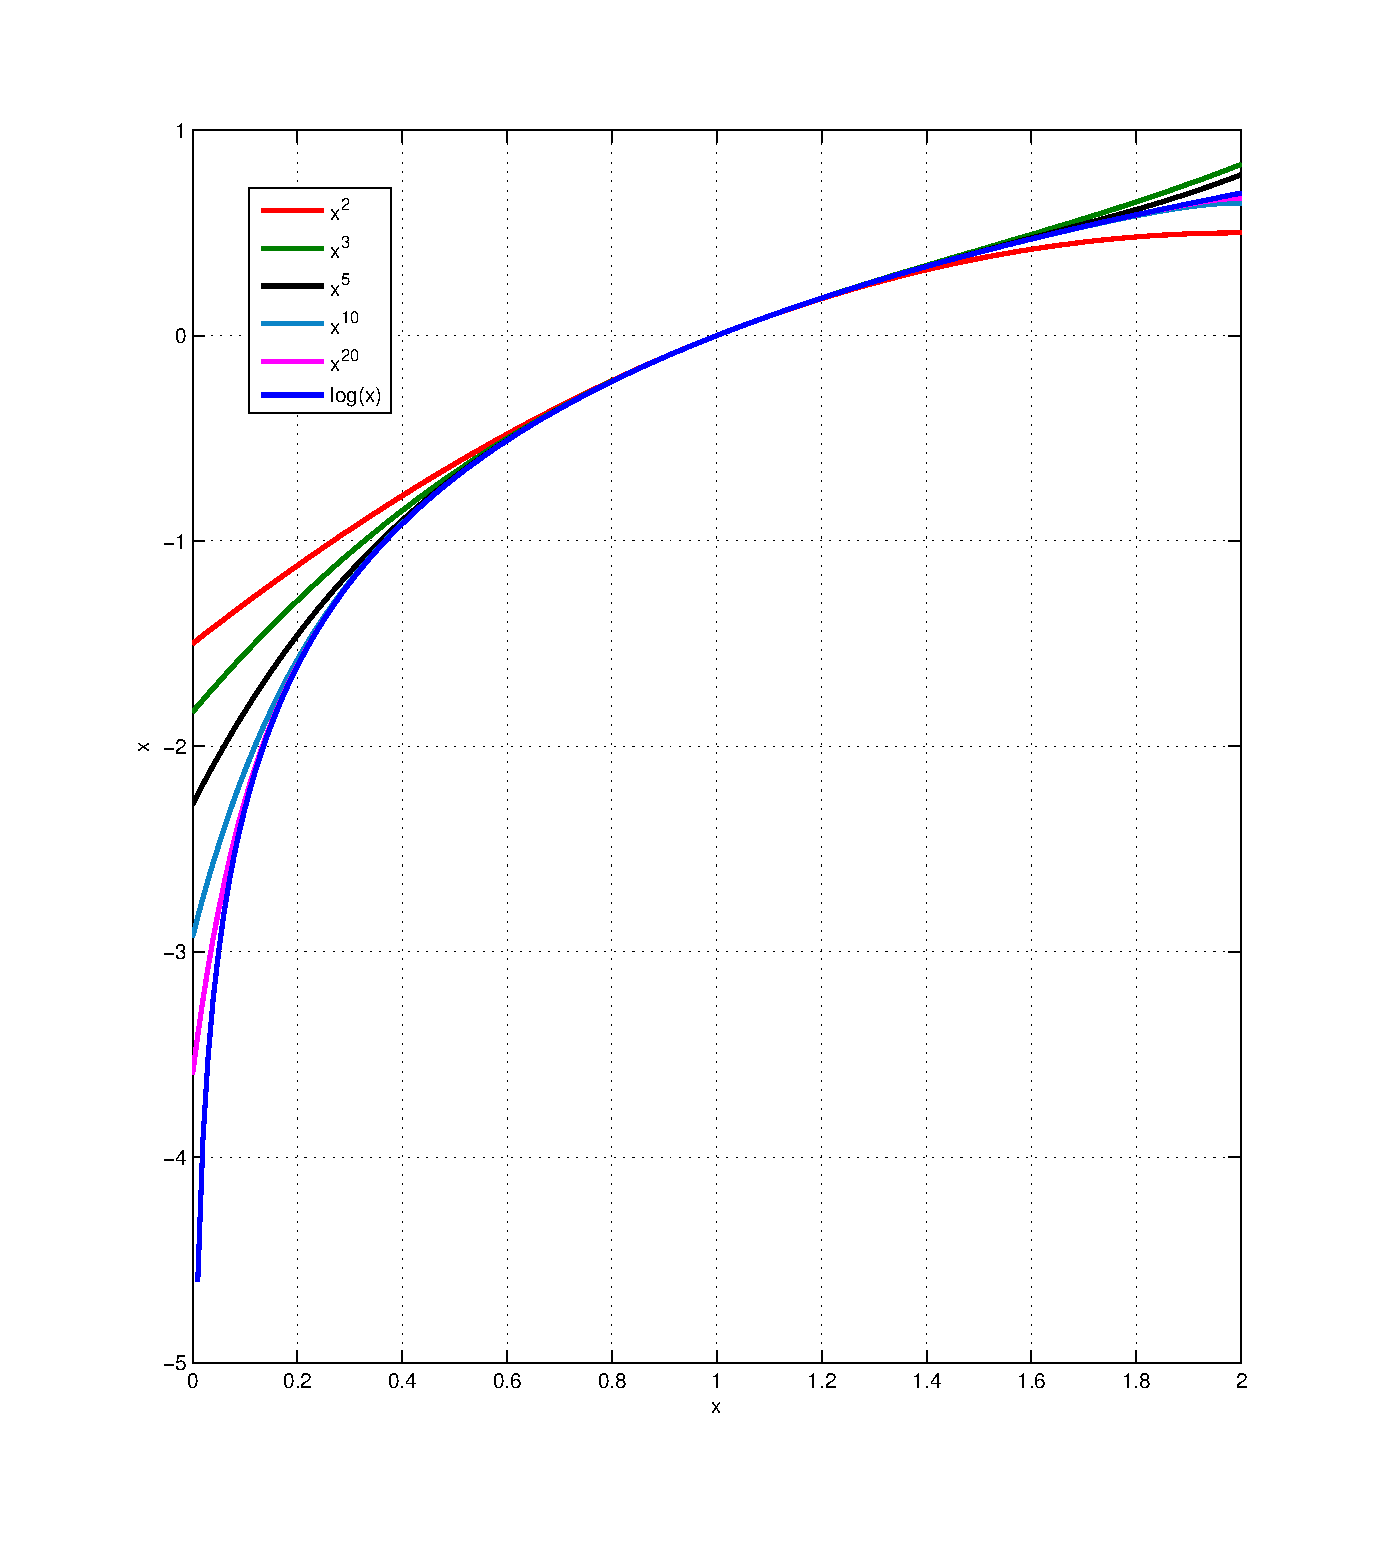
\includegraphics[width=10cm]{ln.eps}
\bicaption{Comparación entre resultados obtenidos para polinomios de Taylor del logaritmo natural. (grados 2, 3, 5, 10, 20)}{A comparison among the results achieved using Taylor polynomials to approach the logarithm. (2, 3, 5, 10, 20 degrees)  }
\label{fig:ln}
\end{figure}
\begin{paracol}{2}
\index{Polinomio de Taylor! Series de las funciones seno y coseno}
Las funciones $\sin(x)$ y $\cos(x)$, son también simples de aproximar mediante polinomios de Taylor. Si desarrollamos en torno a $x_0=0$, la serie del coseno solo tendrá potencias pares mientras que la del seno solo tendrá potencias impares,
\switchcolumn
\index[eng]{Tailor's polynomial! Sine and consine function expansion.} Functions $\sin(x)$ and $\cos(x)$, are also easy to approach using Taylor's polynomials. If we expand around $x_0=0$, the cosine series will have only even powers and the sine series will only have odd powers,
\end{paracol}
\begin{align*}
	\cos(x)&\approx \sum_{i=0}^n \frac{(-1)^i}{(2i)!}x^{2i}\\
	\sin(x)&\approx \sum_{i=0}^n \frac{(-1)^i}{(2i+1)!}x^{2i+1}
\end{align*}

\begin{figure}
	\centering
	\subfigure[$\cos(x)$, polinomios 2, 4, 6 y 8 grados \textreferencemark\ polynomials 2, 4, 6 and 8 degrees  \label{fig:cos}]{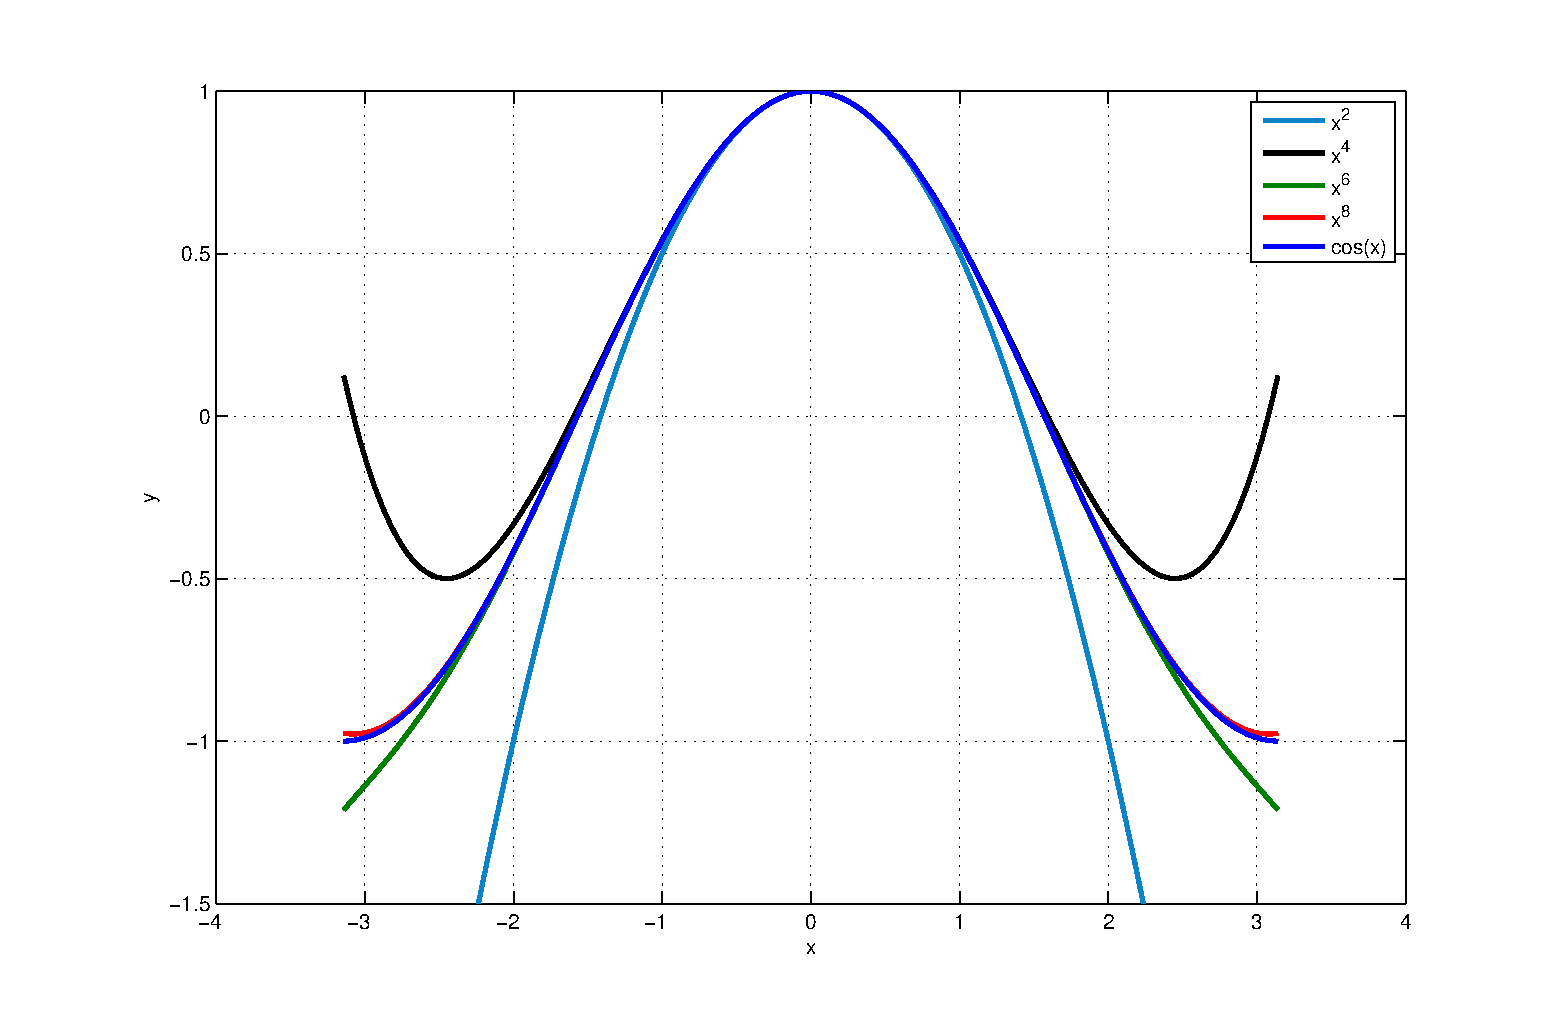
\includegraphics[width=10.5cm]{cos.eps}} \qquad 
	\subfigure[$\sin(x)$, polinomios  3, 5, 7 y 9  grados \textreferencemark polynomials 2, 4, 6 and 8 degrees \label{fig:sin}]{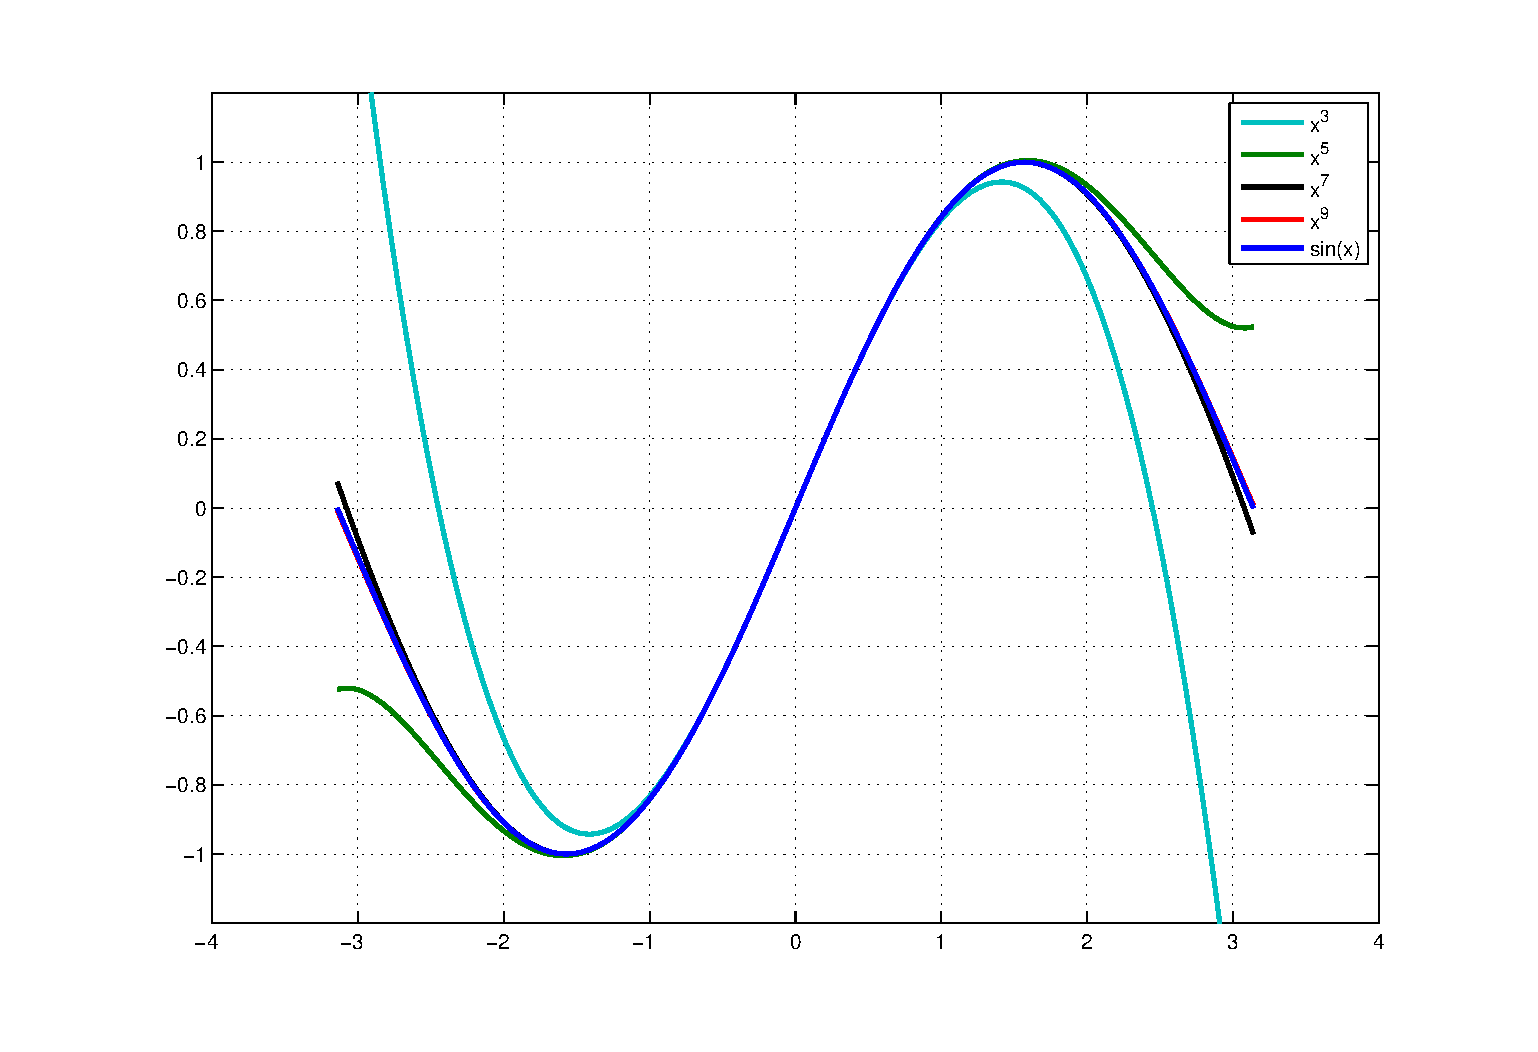
\includegraphics[width=10.5cm]{sin.eps}}\\
	\bicaption{Polynomios de Taylor para las funciones coseno y seno}{Taylor polynomial for cosine and sine functions}
\end{figure}


\begin{paracol}{2}
En las figuras \ref{fig:cos} y \ref{fig:sin} Se muestran las aproximaciones mediante polinomios de Taylor de las funciones coseno y seno. Para el coseno se han empleado polinomios hasta grado 8 y para el seno hasta grado 9. En ambos casos se dan los resultados correspondientes a un periodo $(-\pi, \pi)$. Si se comparan los resultados con las funciones \texttt{cos} y \texttt{sin}, suministradas por Numpy, puede observarse que la aproximación es bastante buena para los polinomios de mayor grado empleados en cada caso.

\section{Interpolación polinómica.}
\sectionmark{Interpolación polinómica \textreferencemark\ Polynomial interpolation}

Se entiende por interpolación el proceso por el cual, dado un conjunto de pares de puntos $(x_0,y_0),(x_1,y_1),\cdots (x_n,y_n)$ se obtiene una función $f(x)$, tal que, $y_i=f(x_i)$, para cada par de puntos $(x_i,y_i)$ del conjunto. Si, en particular, la función empleada es un polinomio $f(x)\equiv p(x)$, entonces se trata de interpolación polinómica. \index{Interpolación! Polinómica}

\paragraph{Teorema de unicidad.} Dado un conjunto \index{Interpolación! Teorema de unicidad}  $(x_0,y_0),(x_1,y_1),\cdots (x_n,y_n)$ de $n+1$ pares de puntos, tales que todos los valores $x_i$ de dicho conjuntos son diferentes entre sí, solo existe un polinomio $p(x)$ de grado $n$, tal que $y_i=p(x_i)$ para todos los pares de puntos del conjunto.

Si tratamos de interpolar los puntos con un polinomio de grado menor que $n$, es posible que no encontremos ninguno que pase por todos los puntos. Si, por el contrario empleamos un polinomio de grado mayor que $n$, nos encontramos con que no es único. Por último si el polinomio empleado es de grado $n$, entonces será siempre el mismo con independencia del método que empleemos para construirlo.

\subsection{La matriz de Vandermonde} \index{Matriz de Vandermonde}
Supongamos que tenemos un conjunto de pares de puntos $\mathcal{A}$, 

\switchcolumn
Figures \ref{fig:cos} and \ref{fig:sin} show aproximations to sine and consine functions using Taylor's polynomials. We have use polynomias up to 8 degree for the cosine function and up to degree 9 for the sine function. In both cases we have calculated the results inside the interval $(-\pi, \pi)$. When we compare these results with those yielded by Numpy functions \mintinline{python}{cos} and \mintinline{python}{sin}, we see that the approximation is quite good for the higher degree  polynomials we have used in each case.

\section{Polynomial interpolati\-on.}
\sectionmark{Interpolación polinómica  \textreferencemark\ Polynomial interpolation}
We define the interpolation as a process that, departing from a set of data pairs \\ $(x_0,y_0),(x_1,y_1), \cdots (x_n,y_n)$, allows us to find a function $f(x)$ such that $y_i = f(x_i)$ for all pairs $(x_i,y_i)$ of the set. In the case we use a polynomial as the interpolating function $f(x)\equiv p(x)$, we denote it as polynomial Interpolation. \index{Interpolation! Polynomial}

\paragraph{The interpolation theorem.}\index[eng]{Interpolation! Interpolation theorem}
For any set of $n+1$ pairs of data points\\ $(x_0,y_0) ,(x_1,y_1),\cdots (x_n,y_n)$ , where no two $x_i$ are the same, there is one and only one polynomial $p(x)$ of degree $n$ that interpolates these points, i.e, it satisfies that $y_i=p(x_i)$ for all pairs on the dataset.

If we try to interpolate the points with a polynomial whose degree is less than $n$, it is possible that we will not find one that fits all the pairs in the dataset. Conversely, if we try to use a polynomial with a degree greater than $n$, it will not unique. Eventually, if we use a degree $n$ polynomial, this polynomial is always the same regardless method used to build it.        

\subsection{The Vandermonde's matrix}\index[eng]{Intrpolation! Vandermonde's matrix}
Suppose we have a set $\mathcal{A}$ of data points.
\end{paracol}
\begin{table}[h]
%\caption{$f(x)=erf(x)$}
\centering
\begin{tabular}{c|c}
$x$&$f(x)$\\ 
\hline
$x_0$& $y_0$\\
$x_1$&$y_1$\\
$x_2$&$y_2$\\
$\vdots$&$\vdots$\\
$x_n$&$y_n$
\end{tabular}
\label{tpuntos3}
\end{table}
\begin{paracol}{2}
Para que un polinomio de orden $n$,

\switchcolumn
For a polynomial of degree $n$,
\end{paracol}
\begin{equation*}
p(x)=a_0+a_1x+a_2x^2+\cdots+a_nx^n
\end{equation*}
\begin{paracol}{2}
pase por todos los pares de $\mathcal{A}$ debe cumplir,
\switchcolumn
to go through all pairs in $\mathcal{A}$, it must satisfy,
\end{paracol}
\begin{equation*}
y_i=a_0+a_1x_i+a_2x_i^2+\cdots+a_nx_i^n, \ \forall (x_i,y_i) \in \mathcal{A}
\end{equation*}
\begin{paracol}{2}
Es decir, obtendríamos un sistema de $n$ ecuaciones lineales, una para cada par de valores, en la que las incógnitas son precisamente los $n+1$ coeficientes $a_i$ del polinomio.

Por ejemplo para los puntos,
\switchcolumn
So, we would have a system of $n$ linear equations, one for each pair of data points, where the unknowns are the $n+1$ coefficients $a_i$ of the polynomial.

for example, for the dataset,  

\end{paracol}
\begin{table}[h]
%\caption{$f(x)=erf(x)$}
\centering 
\begin{tabular}{c|c}
$x$&$f(x)$\\ 
\hline
$1$&$\ 2$\\
$2$&$ \ 1$\\
$3$&$-2$
\end{tabular}
\label{tpuntos4}
\end{table}
\begin{paracol}{2}
Obtendríamos,
\switchcolumn
we get,
\end{paracol}
\begin{align*}
a_0+a_1\cdot 1+ a_2\cdot 1^2&=2\\
a_0+a_1\cdot 2+ a_2\cdot 2^2&=1\\
a_0+a_1\cdot 3+ a_2\cdot 3^2&=-2
\end{align*}
\begin{paracol}{2}
que podríamos expresar en forma matricial como,
\switchcolumn
which we can express in matrix form as,
\end{paracol}

\begin{equation*}
\begin{pmatrix}
1&1&1^2\\
1&2&2^2\\
1&3&3^2
\end{pmatrix}\cdot \begin{pmatrix}
a_0\\
a_1\\
a_2
\end{pmatrix}=\begin{pmatrix}
2\\
1\\
-2
\end{pmatrix}
\end{equation*}
\begin{paracol}{2}
Y en general, para $n$ pares de datos,
\switchcolumn
And, in general, for $n$ data pairs,
\end{paracol}
\begin{equation*}
\begin{pmatrix}
1&x_0&x_0^2&\cdots &x_0^n\\
1&x_1&x_1^2&\cdots &x_1^n\\
\vdots&\vdots&\vdots&\ddots&\vdots\\
1&x_n&x_n^2&\cdots &x_n^n
\end{pmatrix}\cdot \begin{pmatrix}
a_0\\
a_1\\
\vdots\\
a_n

\end{pmatrix}=\begin{pmatrix}
y_0\\
y_1\\
\vdots\\
y_n
\end{pmatrix}
\end{equation*}
\begin{paracol}{2}
La matriz de coeficientes del sistema resultante recibe el nombre de matriz de Vandermonde. Está formada por la $n$ primeras potencias de cada uno de los valores de la variable independiente, colocados por filas. Es evidente que cuanto mayor es el número de datos, mayor tenderá a ser la diferencia de tamaño entre los elementos de cada fila. Por ello, en la mayoría de los casos, resulta ser una matriz mal condicionada para resolver el sistema numéricamente. En la práctica, para obtener el polinomio interpolador, se emplean otros métodos alternativos,

\subsection{El polinomio interpolador de Lagrange.} \label{sec:lagranje}\index{Interpolación! Polinomio de Lagrange} \index{Polinomio de Lagrange}

A partir de los valores $x_0, x_1,\cdots, x_n$, se construye el siguiente conjunto de $n+1$ polinomios de grado $n$

\switchcolumn
The coefficient matrix of the resulting system is called the Vandermonde's matrix. Its elements are hte $n$ first powers of the independent variable values, allocated by rows. It is easy to notice that when the number of data increases the difference among the elements of a row will tend to increase also. For this reason in most cases the Vandermonde's matrix is a poor conditioned matrix and so not suitable for solving the system numerically.  For this reason, in practice,the interpolation polynomial is computed using other alternative methods.  

\subsection{Lagrange Interpolating Polynomial}\index[eng]{Interpolation!Lagrange Polynomial} \index[eng]{Lagrange Polynomial}
Departing from the values $x_0,x_1,\cdots,x_n$, We build the following set of $n+1$ polynomial of degree $n$ 
\end{paracol}
\begin{equation*}
l_j(x)=\prod_{\substack{k=0\\
k\neq j}}^n\frac{x-x_k}{x_j-x_k}=\frac{(x-x_0)(x-x_1)\cdots(x-x_{j-1})(x-x_{j+1})\cdots(x-x_n)}{(x_j-x_0)(x_j-x_1)\cdots(x_j-x_{j-1})(x_j-x_{j+1})\cdots(x_j-x_n)}
\end{equation*}
\begin{paracol}{2}
Los polinomios así definidos cumplen una interesante propiedad en  relación con los valores $x_0, x_1,\cdots, x_n$, empleados para construirlos,
\switchcolumn
These polynomial exhibit an interesting property when evaluated at the points $x_0, x_1,\cdots, x_n$, we have used for building them.
\end{paracol}
\begin{equation*}
l_j(x_i)= \left\{ 
\begin{aligned}
1,\ i=j\\
0,\ i\neq j
\end{aligned}
\right.
\end{equation*}
\begin{paracol}{2}
A partir de estos polinomios podemos construir ahora el siguiente polinomio de interpolación empleando las imágenes $y_0,y_1\cdots, y_n$ correspondientes a los valores $x_0, x_1,\cdots, x_n$,
\switchcolumn
From this polynomials we can build a interporlation polynomial using the codomain values $y_0,y_1\cdots, y_n$  corresponding to the domain values $x_0, x_1,\cdots, x_n$,
\end{paracol}
\begin{equation*}
p(x)=\sum_{j=0}^n l_j(x)\cdot y_j
\end{equation*}
\begin{paracol}{2}
Efectivamente, es fácil comprobar que, tal y como se ha construido, este polinomio pasa por los pares de puntos $x_i,y_i$, puesto que $p(x_i)=y_i$.

El siguiente código de en Python calcula el valor en un punto x cualquiera del polinomio de interpolación de Lagrange construido a partir un conjunto de puntos $\mathcal{A}\equiv \{(x_i,y_i)\}$.
\switchcolumn
It is ease to check that, using this method for building the interpolation polynomial, it passes through all pairs of points $x_i,y_i$, because $p(x_i)=y_i$.

The following python function \mintinline{python}{lagrang} calculates, at any point x, the Lagrange interpolating polynomial value built from a set of pairs of points $\mathcal{A}\equiv \{(x_i,y_i)\}$.   
\end{paracol}

\inputminted[
frame=lines,
framesep=2mm,
baselinestretch=1.2,
%bgcolor=LightGray,
label=lgr\_pol.py,
fontsize=\footnotesize,
linenos
]{python}{./codigos/interpolacion/lgr_pol.py}

\begin{paracol}{2}
\subsection{Diferencias divididas.}\label{sec:difdiv} \index{Interpolación! Diferencias Divididas} \index{Diferencias Divididas}
Tanto el método de la matriz de Vandermonde como el de los polinomios de Lagrange, presentan el inconveniente de que si se añade un dato más $(x_{n+1}, y_{n+1})$ a la colección de datos ya existentes, es preciso recalcular el polinomio de interpolación desde el principio. 

El método de las diferencias divididas, permite obtener el polinomio de interpolación en un número menor de operaciones que en el caso del polinomio de Lagrange y además, el cálculo se hace escalonadamente, aprovechando todos los resultados anteriores cuando se añade al polinomio la contribución de un nuevo dato.

El polinomio de orden $n$ de diferencias divididas se construye de la siguiente manera,
\switchcolumn
\subsection{Divided diferences.}\index{Interpolation! Divided diferences} \index{Divided diferences}
The two method we have studied so far, Vadermonde matrix and Lagrange polynomial, have a common drawback. If we add a new pair of data $(x_{n+1},y_{n+1})$ to the existing data collection, it is necessary to recalculate the interpolation polynomial from scratch.

The divided differences algorithm allows us to build the interpolation polynomial performing less operations than in the case of Lagrange polynomial. Besides, the computing is carried out stepwise, making use of all previous results when a new data  pair is added to calculate the interpolation polynomial.

We build the divided differences polynomial of degree $n$ as follows, 
\end{paracol}
\begin{equation*}
p_n(x)=a_0+(x-x_0)\cdot a_1+(x-x_0)\cdot (x-x_1)\cdot a_2+\cdots +(x-x_0)\cdot (x-x_1)\cdots (x-x_{n-2})\cdot(x-x_{n-1})\cdot a_n
\end{equation*}

\begin{paracol}{2}
Donde, $(x_0, y_0), (x_1,y_1), \cdots (x_n, y_n)$, representan los datos para los que se quiere calcular el polinomio interpolador de grado $n$. Si sustituimos las datos en el polinomio, llegamos a un sistema de ecuaciones, triangular inferior, en el que las incógnitas son los coeficientes del polinomio.
\switchcolumn
Where $(x_0, y_0), (x_1,y_1), \cdots (x_n, y_n)$, represent the dataset for which we want to calculate the interpolation polynomial of degree $n$. If we evaluate the polynomial using the dataset we arrive to a lower triangular system of linear equation, where the polynomial coefficients are the unknowns.    
\end{paracol}
\begin{align*}
a_0&&=y_0\\
a_0&+(x_1-x_0)a_1&=y_1\\
a_0&+(x_2-x_0)a_1+(x_2-x_0)(x_2-x_1)a_2&=y_2\\
\cdots\\
a_0&+(x_n-x_0)a_1+\cdots+(x_n-x_0)(x_n-x_1)\cdots (x_n-x_{n-2})(x_n-x_{n-1})a_n&=y_n
\end{align*}
\begin{paracol}{2}
Este sistema se resuelve explícitamente empleando un esquema de diferencias divididas. 

La diferencia divida de primer orden entre dos puntos $(x_0,y_0)$ y $(x_1,y_1)$ se define como,
\switchcolumn
This system can be solved using the divided differences algorithm.

We define the first-order two-point divided difference $(x_0,y_0)$ y $(x_1,y_1)$ as, 
\end{paracol}
\begin{equation*}
f\left[x_0,x_1\right]=\frac{y_1-y_0}{x_1-x_0}
\end{equation*}														
\begin{paracol}{2}
Para tres puntos, $(x_0,y_0)$, $(x_1,y_1)$ y $(x_2,y_2)$, se define la diferencia dividida de segundo orden como,  
\switchcolumn
For three point, $(x_0,y_0)$, $(x_1,y_1)$ y $(x_2,y_2)$, we define the second-order divided  difference as, 
\end{paracol}
\begin{equation*}
f\left[x_0,x_1,x_2\right]=\frac{f\left[x_1,x_2\right]-f\left[x_0,x_1\right]}{x_2-x_0}
\end{equation*}
\begin{paracol}{2}
y, en general definiremos la diferencia dividida de orden $i$ para $i+1$ puntos como,
\switchcolumn
and eventually, we can define the $i-\text{order}$ divide diference for $i+1$ points as,
\end{paracol}
\begin{equation*}
f\left[x_0,x_1,\cdots,x_i\right]=\frac{f\left[x_1,x_2,\cdots,x_i\right]-f\left[x_0,x_1,\cdots,x_{i-1}\right]}{x_i-x_0}
\end{equation*}																					\begin{paracol}{2}	
Si despejamos por sustitución progresiva los coeficientes del polinomio de interpolación del sistema triangular inferior obtenido, cada coeficiente puede asociarse a una diferencia dividida,
\switchcolumn
We can now get the polynomial coefficients applying progressive substitutions to the lower triangular system defined above, then, each coefficient may be related with a divided difference, 
\end{paracol}
\begin{align*}
a_0&=f\left[x_0\right]=y_0\\
a_1&=f\left[x_0,x_1\right]\\
\vdots\\
a_i&=f\left[x_0,x_1,\cdots,x_i\right]\\
\vdots\\
a_n&=f\left[x_0,x_1,\cdots,x_n\right]\\
\end{align*}																					\begin{paracol}{2}			
Por tanto, podemos obtener directamente los coeficientes del polinomio calculando las diferencias divididas. Veamos un ejemplo empleando el siguiente conjunto de cuatro datos,
\switchcolumn
Therefore we can get the polynomial coefficients straightforwardly if we compute the divided differences. Let's see an example using the following four data set. 
\end{paracol}
\begin{table}[h]
\centering
\begin{tabular}{c|cccc}
x&0&1&3&4\\
\hline
y&1&-1&2&3
\end{tabular}
\end{table}
\begin{paracol}{2}
Habitualmente, se construye a partir de los datos una tabla, como la  \ref{tabdif}, de diferencias divididas. Las primera columna contiene los valores de la variable $x$, la siguiente los valores de las diferencias divididas de orden cero (valores de $y$). A partir de la segunda, las siguientes columnas contienen las diferencias dividas de los elementos de la columna anterior, calculados entre los elementos que ocupan filas consecutivas. La tabla va perdiendo cada vez una fila, hasta llegar a la diferencia dividida de orden $n-1$ de todos los datos iniciales.
\switchcolumn
Usually, we build the divided difference polynomial, using a table such as table \ref{tabdif}. the first column contains the values of variable $x$ the second the values of the cero-order divided differences (values of variable $y$). From the second one on, the following columns contain the divided differences of the elements held in the  previous column. These differences are calculated using the elements located on consecutive rows. The table lost a row each time we advance a column. When we arrive to the $n-1$-order divided difference, we have a single value that depends on all initial data.     
\end{paracol}
\begin{table}[h]
\centering
\bicaption{Tabla de diferencia divididas para cuatro datos}{four data divided difference table}
\begin{tabular}{ccccc}
$x_i$&$y_i$&$f\left[x_i,x_{i+1}\right]$&$f\left[x_i,x_{i+1},x_{i+2}\right]$&$f\left[x_i,x_{i+1},x_{i+2},x_{i+3}\right]$\\
\hline
$x_0=0$&$y_0=\ \  1$&$f\left[x_0,x_1\right]=-2$&$f\left[x_0,x_1,x_2\right]=\ \ 7/6$&$f\left[x_0,x_1,x_2,x_3\right]=-1/3$\\
$x_1=1$&$y_1=-1$&$f\left[x_1,x_2\right]=3/2$&$f\left[x_1,x_2,x_3\right]=-1/6$\\
$x_2=3$&$y_2=\ \ 2$&$f\left[x_2,x_3\right]=\ \ 1$\\
$x_3=4$&$y_3=\ \ 3$\\

\end{tabular}
\label{tabdif}
\end{table}
\begin{paracol}{2}
Los coeficientes del polinomio de diferencias divididas se corresponden con los elementos de la primera fila de la tabla. Por lo que en nuestro ejemplo el polinomio resultante sería,
\switchcolumn
The divided differences polynomial coefficients are the elements held in the first row of the table. So, for our example, we obtain the following interpolation polynomial, 
\end{paracol}
\begin{equation*}
p_3(x)=1-2x+\frac{7}{6}x(x-1)-\frac{1}{3}x(x-1)(x-3)
\end{equation*}
\begin{paracol}{2}
Es importante hacer notar que el polinomio de interpolación obtenido por diferencias divididas siempre aparece representado como suma de productos de binomios $(x-x_0)(x-x_1)\cdots$ y los coeficientes obtenidos corresponden a esta representación y no a la representación habitual de un polinomio como suma de potencias de la variable $x$. 

El siguiente código permite calcular el polinomio de diferencias divididas a partir de un conjunto de $n$ datos. Como el polinomio de diferencias divididas toma una forma especial, es preciso tenerlo en cuenta a la hora de calcular su valor en un punto $x$ determinado. La función \mintinline{python}{difdiv} permite obtener los coeficientes del polinomio de diferencias divididas a partir de una coleccion de datos $x,y$. La función \mintinline{python}{evdif} permite calcular el valor que toma el polinomio en un punto cualquiera $x_i$, a partir de los coeficientes calculados y los valores $x$ de la collección de datos.
\switchcolumn
Notice that the interpolation polynomial, built using divided differences, it always represented as a sum of binomials products $(x-x_0)(x-x_1)\cdots$ and the coefficients computed belong to this representation a not to the standard polynomial representation as a sum of variable $x$ powers.

The following code implement the divided differences polynomial from a set of $n$ data. We must take into account the special form of the polynomial to calculate the value ot takes in an specific $x$ point. Function \mintinline{python}{difdiv} computes the polynomiañ coefficients departing from a set $x,y$ of data. Function \mintinline{python}{evdif} calculates the value of the polynomial in a point whatsoever, using the computed coefficientes and the $x$ values of the data set.  
\end{paracol}

\inputminted[
frame=lines,
framesep=2mm,
baselinestretch=1.2,
%bgcolor=LightGray,
label=dif\_div.py,
fontsize=\footnotesize,
linenos
]{python}{./codigos/interpolacion/dif_div.py}
\begin{paracol}{2} 
 \subsection{El polinomio de Newton-Gregory} \label{sec:newgre} \index{Interpolación!Polinomio de Newton-Gregory} \index{Polinomio de Newton-Gregory}
 Supone una simplificación al cálculo del polinomio de diferencias divididas para el caso particular en que los datos se encuentran equiespaciados y dispuestos en orden creciente con respecto a los valores de la coordenada $x$.
 
En este caso, calcular los valores de las diferencias es mucho mas sencillo.  Si pensamos en las diferencias de primer orden, los denominadores de todas ellas son iguales, puesto que los datos están equiespaciados,
\switchcolumn
\subsection{The Newton-Gregory polynomial}\index[eng]{Interpolation!The Newton-Gregory polynomial}\index[eng]{The Newton-Gregory polynomial}
This polynomial is a simplification of the divided difference polynomial for the case in which the $x$ data of the data set are equispaced and increasingly ordered.

For this case, it is much easier to compute the values of the differences. Think, for instance, in the first-order differences, as far as the data are equispaced ll denominators are equal,  
\end{paracol}
\begin{equation*}
\Delta x \equiv x_i-x_{i-1} =h
\end{equation*}
\begin{paracol}{2}
En cuanto a los numeradores, se calcularían de modo análogo al de las diferencias divididas normales,
\switchcolumn
Concerning the numerators, they are computed as in the standard case of divided differences,
\end{paracol}
\begin{equation*}
\Delta y_0= y_1-y_0, \Delta y_1=y_2-y_1, \cdots, \Delta y_i=y_{i+1}-y_i, \cdots, \Delta y_{n-1}=y_{n}-y_{n-1}
\end{equation*}
\begin{paracol}{2}
Las diferencias de orden superior para los numeradores se pueden obtener de modo recursivo, a partir de las de orden uno, puesto que los denominadores de todas ellas $h$, son iguales.
\switchcolumn
Higher order differences can be computed recursively from the first-order differences because the denominator of them all, $h$ are equal.
\end{paracol}

\begin{equation*}
\Delta^2 y_0=\Delta \left(\Delta y_0 \right) =(y_2-y_1)-(y_1-y_0)=(y_2-2y_1+y_0)
\end{equation*}
\begin{paracol}{2}
En este caso, el denominador de la diferencia sería $x_2-x_0=2h$, y la diferencia tomaría la forma,
\switchcolumn
In this case, the difference denominator would be $x_2-x_0=2h$, and the difference would take the form,  
\end{paracol}
\begin{equation*}
f[x_0,x_1,x_2]=\frac{\Delta^2y_0}{2h^2}
\end{equation*}
\begin{paracol}{2}
En general, para la diferencias de orden n tendríamos,
\switchcolumn
In genral, for the order-n differences we obtain,

\end{paracol}
\begin{equation*}
\Delta^n y_0=y_n-\binom{n}{1}\cdot y_{n-1}+\binom{n}{2}\cdot y_{n-2}-\cdots+(-1)^n\cdot y_0
\end{equation*}
\begin{paracol}{2}
Donde se ha hecho uso de la expresión binomial,
\switchcolumn
Where we have used the binomial expression,
\end{paracol}
\begin{equation*}
\binom{k}{l}=\frac{k!}{l!\cdot(k-l)!}
\end{equation*}
\begin{paracol}{2}
Para obtener la diferencia dividida de orden n, bastaría ahora dividir por $n!\cdot h^n$.
\switchcolumn
And, eventually, we obtain the order-n divided difference just dividing by  $n!\cdot h^n$.
\end{paracol}
\begin{equation*}
f\left[x_0,x_1,\cdots,x_n\right]=\frac{\Delta^n y_0}{n!\cdot h^n}
\end{equation*}
\begin{paracol}{2}
A partir de las diferencias, podemos representar el polinomio de diferencias divididas resultante como,
\switchcolumn
Once we have got the differences we can write the divided differences polynomial as,

\end{paracol}
\begin{equation*}
p_n(x)=y_0+\frac{x-x_0}{h}\Delta y_0+\frac{(x-x_1)\cdot (x-x_0)}{2\cdot h^2}\Delta^2 y_0+\cdots +\frac{(x-x_{n-1}) \cdots (x-x_1)\cdot (x-x_0)}{n! \cdot h^n}\Delta^n y_0
\end{equation*}
\begin{paracol}{2}
Este polinomio se conoce como el polinomio de Newton-Gregory, y podría considerarse como una aproximación  numérica al polinomio de Taylor de orden n de la posible función asociada a los datos empleados.

En este caso, podríamos construir la tabla para obtener los coeficientes del polinomio, calculando en cada columna simplemente las diferencias de los elementos de la columna anterior. Por ejemplo,
\switchcolumn
This polynomial is known as the Newton-Gregory polynomial, and it could be considered as a numerical approximation to the n-degree Taylor polynomial of the (possible) function associated to the dataset. 

In this case, we can build the table to  obtain the polynomial coefficients, computing in each column just the differences of the previous column. For example,  
\end{paracol}
\begin{table}[h]
\centering
\bicaption{Tabla de diferencias para el polinomio de Newton-Gregory de cuatro datos}{Table of differences for a Newton-Gregory polynomial of four data}
\begin{tabular}{ccccc}
$x_i$&$y_i$&$\Delta y_i$&$\Delta^2 y_i$&$\Delta^3 y_i$\\
\hline
$x_0=0$&$y_0=\ \  1$&$-2$&$\ \ 5$&$-7$\\
$x_1=1$&$y_1=-1$&$ \ \ 3$&$ -2$\\
$x_2=2$&$y_2=\ \ 2$&$\ \ 1$\\
$x_3=3$&$y_3=\ \ 3$\\

\end{tabular}
\label{tabnewton}
\end{table}
\begin{paracol}{2}
Una vez calculadas las diferencias, basta dividir por $n!\cdot h^n$ los elementos de la primera fila de la tabla,
\switchcolumn
Once we have computed the differences, it is enough to divide by $n!\cdot h^n$ the elements of the table first row, 
\end{paracol}
\begin{equation*}
a_0=1, a_1=\frac{-2}{1}, a_2=\frac{5}{2\cdot 1^2}, a_3=\frac{-7}{6\cdot 1^3}
\end{equation*}
\begin{paracol}{2}
El siguiente código muestra un ejemplo de implementación en Python del polinomio de Newton-Gregory
\switchcolumn
The following code shows an example of Python implementation for the Newton-Gregory polynomial
\end{paracol}
\inputminted[
frame=lines,
framesep=2mm,
baselinestretch=1.2,
%bgcolor=LightGray,
label=newton\_gregory.py,
fontsize=\footnotesize,
linenos
]{python}{./codigos/interpolacion/newton_gregory.py}


\begin{figure}[h]
\centering
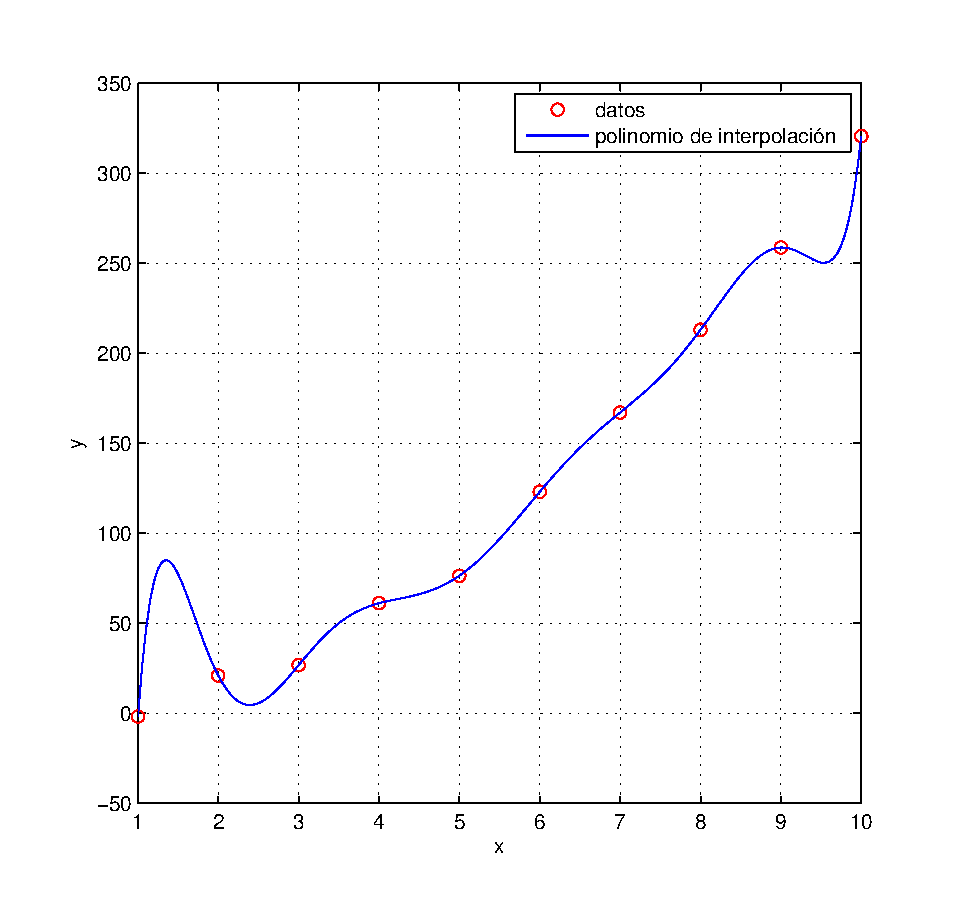
\includegraphics[width=10cm]{intpoli.eps}
\bicaption{Polinomio de interpolación de grado nueve obtenido a partir de un conjunto de diez datos}{Nine degree interpoling polynomial obtained using a set of ten data}
\label{fig:intepol}
\end{figure}
\begin{paracol}{2}
\section{Interpolación por intervalos.}
\sectionmark{Interp. por intervalos \textreferencemark\ Piecewise interpolation}
Hasta ahora, hemos visto cómo interpolar un conjunto de $n+1$ datos mediante un polinomio de grado $n$. En muchos casos, especialmente cuando el número de datos es suficientemente alto, los resultados de dicha interpolación pueden no ser satisfactorios.  La razón es que el grado del polinomio de interpolación crece linealmente con el número de puntos a interpolar, así por ejemplo para interpolar 11 datos necesitamos un polinomio de grado 10. Desde un punto de vista numérico, este tipo de polinomios pueden dar grandes errores debido al redondeo. Por otro lado, y dependiendo de la disposición de los datos para los que se realiza la interpolación, puede resultar que el polinomio obtenido tome una forma demasiado complicada para los valores comprendidos entres los datos interpolados..  

La figura \ref{fig:intepol} muestra el polinomio de interpolación de grado nueve para un conjunto de 10 datos. Es fácil darse cuenta, simplemente observando los datos, que no hay ninguna razón que justifique las curvas que traza el polinomio entre los puntos $1$ y $2$  o los puntos $9$ y $10$, por ejemplo.

\switchcolumn
\section{Piecewise interpolation}
\sectionmark{Interp. por intervalos \textreferencemark\ Piecewise interpolation}
So far, we have seen how to interpolate a set of $n+1$ data using a degree $n$ polynomial. In many case, in particular when the number of data is high, the results of such interpolation could be very poor. The problem comes from the linear increasing of the polynomial degree with the number of data. So, if we want to build the interpolation polynomial for a 11 data, we come up with a 10-degree polynomial. From a numerical point of view, this kinda polynomial are prone to cast large errors due to the rounding process. On the other hand, depending on how data used to compute the interpolation are distributed, the polynomial could take a too complicate shape that hardly can be related with the information held in the dataset.

Figure \ref{fig:intepol} shows a interpolating polynomial of degree nine obtained from a set of ten data. It is easy to realise, just for simple inspection, that there in not reason to justify the polynomial curvature between points $1$ and $2$ or between the points $9$ and $10$.     
\end{paracol}
\begin{figure}
\centering
\subfigure[Interpolación de orden cero / Zero-order interpolation  \label{fig:stepwise}]{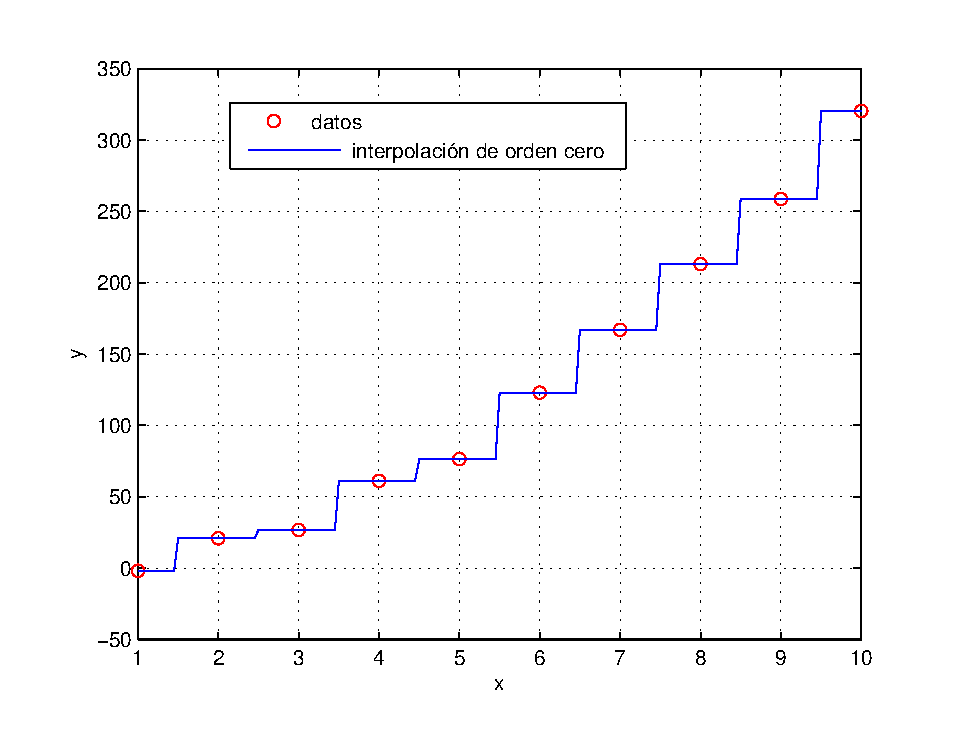
\includegraphics[width=7cm]{steps.eps}} %\qquad 
\subfigure[Interpolación lineal  Linear interpolation  \label{fig:lineal}]{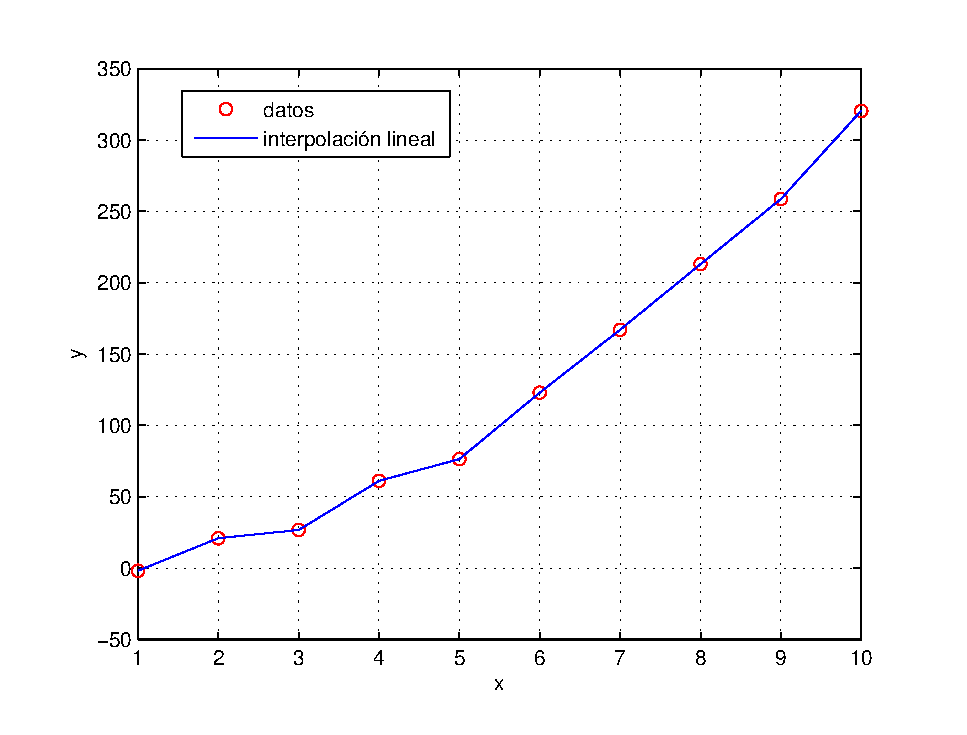
\includegraphics[width=7cm]{lineal.eps}}\\
\bicaption{Interpolaciones de orden cero y lineal para los datos de la figura \ref{fig:intepol} }{Zero-order and linear interpolation for the figure data}
\end{figure}

\begin{paracol}{2}
En muchos casos es preferible no emplear todos los datos disponibles para obtener un único polinomio de interpolación. En su lugar, lo que se hace es dividir el conjunto de datos en varios grupos ---normalmente se agrupan formando intervalos de datos consecutivos--- y obtener varios polinomios de menor grado, de modo que cada uno interpole los datos de un grupo distinto. 

El grado de los polinomios empleados deberá estar, en principio, relacionado con los datos contenidos en cada tramo.


\paragraph{interpolación de orden cero} \index{Interpolación de orden cero} si hacemos que cada intervalo contenga un solo dato, obtendríamos polinomios de interpolación de grado cero, $a_{0i}=y_i$. El resultado, es un conjunto de escalones cuya valor varía de un intervalo a otro de acuerdo con el dato representativo contenido en cada tramo. La figura \ref{fig:stepwise} muestra el resultado de la interpolación de orden cero para los mismos diez datos de la figura \ref{fig:intepol}.

\paragraph{interpolación lineal.} \index{Interpolación lineal} En este caso, se dividen los datos en grupos de dos. Cada par de datos consecutivos se interpola calculando la recta que pasa por ellos. La interpolación lineal se emplea en muchas aplicaciones debido a su sencillez de cálculo. La figura \ref{fig:lineal}, muestra el resultado de aproximar linealmente los mismos datos contenidos en los ejemplos anteriores.

Siguiendo el mismo procedimiento, aumentando el número de datos contenidos en cada intervalo, podríamos definir una interpolación cuadrática, con polinomios de segundo grado, tomando intervalos que contengan tres puntos, una interpolación cúbica, para intervalos de cuatro puntos etc.

\subsection{Interpolación mediante splines cúbicos} \index{Interpolación!Splines}\index{Splines}
Hemos descrito antes cómo el polinomio interpolador de orden $n$ para un conjunto de $n+1$ datos puede presentar el inconveniente de complicar excesivamente la forma de  la curva obtenida entre los puntos interpolados. La interpolación a tramos que acabamos de describir, simplifica la forma de la curva entre los puntos pero presenta el problemas de la continuidad en las uniones entre tramos sucesivos. Sería deseable encontrar métodos de interpolación que fueran capaces de solucionar ambos problemas simultáneamente. Una buena aproximación a dicha solución la proporcionan los \emph{splines}.

Una función \emph{spline} está formada por un conjunto de polinomios, cada uno definido en un intervalo, que se unen entre sí obedeciendo a ciertas condiciones de continuidad.

Supongamos que tenemos una tabla de datos cualquiera,

\switchcolumn
For these reasons, in many cases it is better not to use the whole dataset to build a single interpolation polynomial of maximum degree. Instead, a common practice is to divide the dataset in several groups of data ---usually they are gathered using interval of consecutive data-- and build several polynomial of lower degree, each one interpolating the data of  a different group.

The  degree of the polynomials should be related with the number of data allocated in each interval.

\paragraph{Zero-order interpolation.} \index[eng]{zero-order interpolation} If we get interval which only hold a single  data pair $X,y$, then we get zero-order interpolating polynomials, $a_{0i} = y_i$. The result is a stepwise interpolation which values changes from one interval to the next,  taken the data value defined for each interval according to the dataset.   Figure \ref{fig:stepwise} shows the zero-order interpolation result for the same ten data of figure \ref{fig:intepol}. 

\paragraph{Linear interpolation.} \index[eng]{Linear interpolation} In this case, we divide the dataset in groups of two data. Each two consecutive data are interpolated calculating the line that pass through them. The linear interpolation is very commonly used due to its computing simplicity. Figure \ref{fig:lineal} shows the result of interpolating the same data utilised in previous examples, using linear interpolation. 

Following the same procedure, we can increase the number of data include in each interval and define quadratic interpolation, using second-degree polynomials and taking three points in each interval; cubic interpolation,using  third-degree polynomial and four point intervals. etc.

\subsection{Cubic spline interpolation}\index[eng]{Interpolation!Splines}\index[eng]{Splines}
WE have seen how the $n$-degree interpolating polynomial for a set of $n+1$ data, could present a quite complex shape that does not represent well the information supplied by the dataset. The piecewise interpolation that we have described so far, simplifies the shape of the interpolating curve but have in turn the problem that it loses the continuity in the union between consecutive intervals. It could be valuable to find interpolation methods that may be able to cope with both problems simultaneously. A good approach to solve these problem is supplied by \emph{spline} interpolation. 

A \emph{spline} is function built using a set of polynomials, any one of them defined in an interval. The spline polynomial are connected in the ends of the intervals meeting certain continuity conditions.

Suposse we have a data table whatsoever,
\end{paracol}
\begin{table}[h]
\centering
\begin{tabular}{c|cccc}
x&$x_0$&$x_1$&$\cdots$&$x_n$\\
\hline
y&$y_0$&$y_1$&$\cdots$&$y_n$
\end{tabular}
\end{table}
\begin{paracol}{2}
Para construir una función \emph{spline} $S$ de orden $m$, que interpole los datos de la tabla, se definen intervalos tomando como extremos dos puntos consecutivos de la tabla y un polinomio de grado $m$ para cada uno de los intervalos,
\switchcolumn
To build a $m$ order \emph{spline} function $S$ for interpolating the table data, we define intervals taking two consecutive point onn the table as limits. Then, we define an $m$ degree polynomial for each interval.
\end{paracol}
\begin{equation*}
S= \left\{ 
\begin{aligned}
S_0(x),& \ x\in [x_0,x_1]\\
S_1(x),& \ x\in [x_1,x_2]\\
\vdots \\
S_i(x),& \ x\in [x_i,x_{i+1}]\\
\vdots \\
S_{n-1}(x),& \ x\in [x_{n-1},x_n]
\end{aligned}
\right.
\end{equation*}
\begin{paracol}{2}
Para que $S$ sea una función Spline de orden $m$ debe cumplir que sea continua y tenga $m-1$ derivadas continuas en el intervalo $[x_0,x_n]$ en que se desean interpolar los datos.
   
Para asegurar la continuidad, los polinomios que forman $S$ deben cumplir las siguientes condiciones en sus extremos;
\switchcolumn
For $s$ to be a order $m$ spline function it should be continue and it should have $m-1$ continue derivatives in the interval $[x_0,x_n]$ in which we want to interpolate the data.

To ensure the continuity of the polynomials that build $S$ they must satisfy the following condition at their ends, 
\end{paracol}
\begin{align*}
S_i(x_{i+1})&=S_{i+1}(x_{i+1}),\ (1\leq i \leq n-1)\\
S'_i(x_{i+1})&=S'_{i+1}(x_{i+1}),\ (1\leq i \leq n-1)\\
S''_i(x_{i+1})&=S''_{i+1}(x_{i+1}),\ (1\leq i \leq n-1)\\
\vdots \\
S^{m-1}_i(x_{i+1})&=S^{m-1}_{i+1}(x_{i+1}),\ (1\leq i \leq n-1)\\
\end{align*}
\begin{paracol}{2}
Es decir, dos polinomios consecutivos del spline y sus $m-1$ primeras derivadas, deben tomar los mismos valores en el extremo común. 

Una consecuencia inmediata de las condiciones de continuidad exigidas a los splines es que sus derivadas sucesivas, $S',\ S'', \cdots$ son a su vez funciones spline de orden $m-1,\ m-2, \cdots$. Por otro lado, las condiciones de continuidad suministran  $(n-1)\cdot m$ ecuaciones que, unidas a las $n+1$ condiciones de interpolación ---cada polinomio debe pasar por los datos que constituyen los extremos de su intervalo de definición---,  suministran un total de  $n\cdot (m+1)-(m-1)$ ecuaciones. Este número es insuficiente para determinar los $(m+1)\cdot n$ parámetros correspondientes a los $n$ polinomios de grado $m$ empleados en la interpolación. Las $m-1$ ecuaciones que faltan se obtienen imponiendo a los splines condiciones adicionales.

\paragraph{Splines cúbicos.} \index{Splines! Cubicos} Los splines más empleados son los formados por polinomios de tercer grado. En total, tendremos que determinar $(m+1)\cdot n=4\cdot n$ coeficientes para obtener todos los polinomios que componen el spline. Las condiciones de continuidad más la de interpolación suministran en total $3\cdot (n-1)+n+1=4\cdot n-2$  ecuaciones. Necesitamos imponer al spline dos condiciones más. Algunas típicas son,
\begin{enumerate}
\item Splines naturales $S''(x_0)=S''(x_n)=0$
\item Splines con valor conocido en la primera derivada de los extremos $S'(x_0)=y'_0, S'(x_n)=y'_n$
\item Splines periódicos,
\end{enumerate}
\switchcolumn
That is, two consecutive polynomial belonging to the spline and their $m-1$ first derivatives must take the same values in the common end.

A straightforward consequence of the continuity conditions impose to spline functions is that their successive derivatives $S'.\ S'', \cdots$ are in turn order $m-1, \ m-2 \cdots$ spline functions too. Besides, the continuity conditions supply $(n-1) \cdot m$ equations that, together with the interpolation conditions ---each polynomial should pass through the two data point that defines the ends of its definition interval---, sum up $n\cdot (m+1)-(m-1)$ equations. This number is insufficient for obtaining the $(m+1\cdot n)$ parameters belonging to the the $n$ polynomial of degree $m$ used in the spline interpolation. We need $m-1$ equations more that are defined imposing to the polynomials additional conditions.

\paragraph{Cubic Spline.} Probably, the most used splines are those composed of third-degree polynomials. We must need to determine $(m+1)\dot n = 4\cdot n$ coefficients to obtain all the polynomials that compose the spline. The continuity plus the interpolation conditions supply $3\cdot (n-1)+n+1 = 4\cdot n - 2$ equations. We need to impose two more conditions to the spline. Some frecuently used conditions are,
\begin{enumerate}
	\item natural Spline $S''(x_0)=S''(x_n)=0$
	\item Spline with a known value for the derivatives at the ends of the interval $S'(x_0)=y'_0, S'(x_n)=y'_n$
	\item Periodic Spline,
\end{enumerate}  
\end{paracol}     
\begin{equation*}
\left\{ 
\begin{aligned}
S(x_0)&=S(x_n)\\
S'(x_0)&=S'(x_n)\\
S''(x_0)&=S''(x_n)
\end{aligned}
\right.
\end{equation*}
\begin{paracol}{2}
Intentar construir un sistema de ecuaciones para obtener a la vez todos los coeficientes de todos los polinomios es una tarea excesivamente compleja porque hay demasiados parámetros.  Para abordar el problema partimos del hecho de que $S''(x)$ es también un spline de orden 1 para los puntos interpolados. Si los definimos como,
\switchcolumn
Try to build a system of equations to obtain all the coefficients of all the polynomial at a time, is an arduous task. There are too many parameters. We can address the problem starting with $S''(x)$, which it is also a order-1 spline for the points we want to interpolate. If we define it as,  
\end{paracol}
\begin{equation*}
S''_i(x)=-M_i\frac{x-x_{i+1}}{h_i}+M_{i+1}\frac{x-x_i}{h_i},\   i=0,\cdots, n-1
\end{equation*}

\begin{paracol}{2}
donde $h_i=x_{i+1}-x_i$ representa el ancho de cada intervalo y donde cada valor $M_i=S''(x_i)$ será una de las incógnitas que deberemos resolver.

Si integramos dos veces la expresión anterior,
\switchcolumn
Where  $h_i=x_{i+1}-x_i$ stand for each interval width and where the value $M_i=S''(x_i)$ will be the unknown we have to solve. 

Now, we integrate two times this expression, $S_i''(x)$, to obtain,
\end{paracol}
\begin{align*}
S'_i(x)&=-M_i\frac{(x-x_{i+1})^2}{2\cdot h_i}+M_{i+1}\frac{(x-x_i)^2}{2\cdot h_i}+A_i,\   i=0,\cdots, n-1\\
S_i(x)&=-M_i\frac{(x-x_{i+1})^3}{6\cdot h_i}+M_{i+1}\frac{(x-x_i)^3}{6\cdot h_i}+A_i(x-x_i)+B_i,\   i=0,\cdots, n-1\\
\end{align*}
\begin{paracol}{2}
Empezamos por imponer las condiciones de interpolación: el polinomio $S_i$ debe pasar por el punto $(x_i,y_i)$,

\switchcolumn
Let's start imposing the interpolation conditions: the polynomial $S_i$ must to pass through the point $(x_i,y_i)$,
\end{paracol}
\begin{equation*}
S_i(x_i)=-M_i\frac{(x_i-x_{i+1})^3}{6\cdot h_i}+B_i=y_i \Rightarrow B_i=y_i-\frac{M_i\cdot h_i^2}{6},\ i=0,\cdots, n-1
\end{equation*}
\begin{paracol}{2}
A continuación imponemos continuidad del spline en los nodos comunes: El polinomio $S_{i-1}$ también debe pasar por el punto $(x_i, y_i)$,
\switchcolumn
Then, we impose the continuity of the spline in the points common to two polynomials: Polynomial $S_{i-1}$ must also pass through the point $(x_i, y_i)$, 
\end{paracol}
\begin{align*}
S_{i-1}(x_i)&=M_i\frac{(x_i-x_{i-1})^3}{6\cdot h_i}+A_{i-1}(x_i-x_{i-1})+\overbrace{y_{i-1}-\frac{M_{i-1}\cdot h_{i-1}^2}{6}}^{B_{i-1}}=y_i \Rightarrow\\
\Rightarrow A_{i-1}&=\frac{y_i-y_{i-1}}{h_{i-1}}-\frac{M_i-M_{i-1}}{6}\cdot h_{i-1}, \ i=1,\cdots, n
\end{align*}
\begin{paracol}{2}
Y por tanto,
\switchcolumn
and thus,
\end{paracol}
\begin{equation*}
A_i=\frac{y_{i+1}-y_i}{h_i}-\frac{M_{i+1}-M_i}{6}\cdot h_i, \ i=0,\cdots, n-1
\end{equation*}
\begin{paracol}{2}
En tercer lugar imponemos la condición de que las derivadas también sean continuas en los nodos comunes,
\switchcolumn
Thirdly, we impose that continuity condition to the derivatives, in the common end of two consecutive polynomials,
\end{paracol}
\begin{align*}
S'_i(x_i)&=-M_i\frac{(x_i-x_{i+1})^2}{2\cdot h_i}+M_{i+1}\frac{(x_i-x_i)^2}{2\cdot h_i}+\frac{y_{i+1}-y_i}{h_i}-\frac{M_{i+1}-M_i}{6}\cdot h_i,\   i=0,\cdots, n-1\\
S'_{i-1}(x_i)&=-M_{i-1}\frac{(x_i-x_i)^2}{2\cdot h_{i-1}}+M_{i}\frac{(x_i-x_{i-1})^2}{2\cdot h_{i-1 }}+\frac{y_i-y_{i-1}}{h_{i-1}}-\frac{M_i-M_{i-1}}{6}\cdot h_{i-1},\   i=1,\cdots, n\\
S'_i(x_i)&=S'_{i-1}(x_i) ,\   i=1,\cdots, n-1 \Rightarrow\\
&\Rightarrow -M_i\frac{h_i}{2}+\frac{y_{i+1}-y_i}{h_i}-\frac{M_{i+1}-M_i}{6}\cdot h_i=M_{i}\frac{h_{i-1}}{2}+\frac{y_i-y_{i-1}}{h_{i-1}}-\frac{M_i-M_{i-1}}{6}\cdot h_{i-1}
\end{align*}
\begin{paracol}{2}
Si agrupamos a un lado los valores $M_{i-1}, M_i, M_{i+1}$,

\switchcolumn
If we group at one side the values $M_{i-1}, M_i, M_{i+1}$,
\end{paracol}
\begin{align*}
h_{i-1}\cdot M_{i-1}+2\cdot (h_{i-1}+h_i)\cdot M_i+h_i\cdot M_{i+1}=6\cdot \left(\frac{y_{i+1}-y_i}{h_i}-\frac{y_i-y_{i-1}}{h_{i-1}}\right)\\
i=1,\cdots ,n-1
\end{align*}
\begin{paracol}{2}
En total tenemos $M_0,\cdots, M_n$, $n+1$ incógnitas y la expresión anterior, solo nos suministra $n-1$ ecuaciones. Necesitamos dos ecuaciones más. Si imponemos la condición de splines naturales, para el extremo de la izquierda del primer polinomio y para el extremo de la derecha del último,
\switchcolumn
We have in total  $M_0,\cdots, M_n$, $n+1$ unknowns and the above expression only supply $n-1$ equations. We need two more equations. If we impose the conditions for a natural spline for the left end of the first polynomial and for the right end of the last one,  
\end{paracol}
\begin{align*}
M_0=S''(x_0)=0\\
M_n=S''(x_n)=0
\end{align*}
\begin{paracol}{2}
Con estas condiciones y la expresión obtenida para el resto de los $M_i$, podemos construir un sistema de ecuaciones tridiagonal
\switchcolumn
With these last conditions and the expression obtained for the remaining $M_i$, we can build a tridiagonal system of equations
\end{paracol}
\begin{equation*}
\begin{pmatrix}
2(h_0+h_1) & h_1 & 0 &0&\cdots &0&0\\
 h_1 & 2(h_1+h_2) & h_2 &0& \cdots&0 & 0\\
0& h_2 & 2(h_2+h_3) & h_3 &\cdots &0& 0\\
\vdots & \vdots & \vdots &\vdots& \ddots & \vdots&\vdots \\
0 & 0 & 0&0&\cdots& 2(h_{n-3}+h_{n-2}) & h_{n-2} \\ 
0 & 0 & 0&0&\cdots&h_{n-2} & 2(h_{n-2}+h_{n-1})
\end{pmatrix}\cdot \begin{pmatrix}
M_1\\
M_2\\
M_3\\
\vdots \\
M_{n-1}
\end{pmatrix}=\begin{pmatrix}
b_1\\
b_2\\
b_3\\
\vdots \\
b_{n-1}
\end{pmatrix}
\end{equation*}
\begin{paracol}{2}
Donde hemos hecho,
\switchcolumn
Where,
\end{paracol}
\begin{equation*}
b_i=6\cdot \left(\frac{y_{i+1}-y_i}{h_i}-\frac{y_i-y_{i-1}}{h_{i-1}}\right)
\end{equation*}
\begin{paracol}{2}
Tenemos un sistema de ecuaciones en el que la matriz de coeficientes es tridiagonal y además diagonal dominante, por lo que podríamos emplear cualquiera de los métodos vistos en el capítulo  
\ref{sistemas}.  Una vez resuelto el sistema y obtenidos los valores de $M_i$, obtenemos los valores de $A_i$ y $B_i$ a Partir de las ecuaciones obtenidas más arriba.

Por último, la forma habitual de definir el polinomio de grado 3 $S_i$, empleado para interpolar los valores del intervalo $[x_i,x_{i+1}]$, mediante splines cúbicos se define como, 

\switchcolumn
So, we have a system of equations for which the coefficients matrix is tridiagonal and, besides, it is a dominant diagonal matrix. For this reason, we can solve it with anyone of the methods described in chapter \ref{sistemas}. Once the system is solved, we get the values of $M_i$ and the values of $A_i$ and $B_i$ using the equations described above. 

A last remark: we usually define the 3-degree polynomial, $S_i$ used for interpolating the values inside the interval $[x_i,x_{i+1}]$ as follows, 
\end{paracol}
\begin{equation*}
S_i(x)=\alpha_i+\beta_i(x-x_i)+\gamma_i(x-x_i)^2+\delta_i(x-x_i)^3, \ x\in [x_i,x_{i+1}],\ (i=0,1,\cdots,n-1)
\end{equation*}
\begin{paracol}{2}
Donde,
\switchcolumn
Where,
\end{paracol}
\begin{align*}
\alpha_i &=y_i\\
\beta_i &=\frac{y_{i+1}-y_i}{h_i}-\frac{M_i \cdot h_i}{3}-\frac{M_{i+1} \cdot h_i}{6}\\
\gamma_i &=\frac{M_i}{2}\\
\delta_i &=\frac{M_{i+1}-M_i}{6\cdot h_i}
\end{align*}
\begin{paracol}{2}
La siguiente función permite obtener los coeficientes y el resultado de interpolar un conjunto de puntos mediante splines cúbicos,
\switchcolumn
The following Python code computes the coefficients of the cubic spline defined using a dataset and the value taken by the spline at any point.
\end{paracol}

\inputminted[
frame=lines,
framesep=2mm,
baselinestretch=1.2,
%bgcolor=LightGray,
label=cubic\_spline.py,
fontsize=\footnotesize,
linenos
]{python}{./codigos/interpolacion/cubic_spline.py}

\begin{paracol}{2}
 La figura, \ref{fig:splines} muestra el resultado de interpolar mediante un spline cúbico, los datos contenidos en la figura \ref{fig:intepol}. Es fácil observar cómo ahora los polinomios de interpolación dan como resultado una curva suave en los datos interpolados y en la que además las curvas son también suaves, sin presentar variaciones extrañas, para los puntos contenidos en cada intervalo entre dos datos.
 
\subsection{Funciones propias de Py\-thon para interpolación por intervalos} \index{interp1@\texttt{interp1}}

Para realizar una interpolación por intervalos mediante cualquiera de los procedimientos descritos, podemos emplear el subpaquete de scipy \mintinline{python}{Scipy.interpolate}. Este paquete incorpora múltiples métodos de interpolación; solo veremos dos: 

La función \texttt{interp1d}. Esta función admite como variables de entrada dos arrays con los valores de las coordenadas $x$ e $y$ de los datos que se desea interpolar. Además, admite como variable  de entrada una cadena de caracteres que indica el método con el que se quiere realizar la interpolación. Dicha variable puede tomar los valores:
\begin{enumerate}
\item \texttt{'nearest'}. Interpola el intervalo empleando el valor $y_i$ correspondiente al valor  $x_i$ más cercano al punto que se quiere interpolar. El resultado es una interpolación a escalones.
 del conjunto de datos que se desea interpolar.
\item \texttt{'next'}. Interpola el interpalo empleando el valor de $y_i$ correspondiente al punto $x_i$ de los datos que cierra el intervalo.
\item \texttt{'previous'} Interpola el interpalo empleando el valor de $y_i$ correspondiente al punto $x_i$ de los datos que abre el intervalo.
\item \texttt{'linear'} realiza una interpolación lineal entre los extremos del intervalo que se desea intepolar. Esta es la opción por defecto.
\end{enumerate} 

\mintinline{python}{interp1d} Devuelve una funcion que admite como variable de entrada un array con los puntos para para los que se quiere calcular el valor de la interpolación y devuelve como salidad un array con los resultados obtenidos. El siguiente código muestra el modo de usar el comando \texttt{interp1d}. Para probarlo se han creado dos array \texttt{x} e \texttt{y} que contienen el conjunto de datos que se empleará para calcular la interpolación. Además, se ha creado otro vector \texttt{xi} que contiene los puntos para los que se quiere calcular el resultado de la interpolación.
\switchcolumn
Figure \ref{fig:splines} shows the result of interpolating the same data of figure \ref{fig:intepol} using a cubic spline. It is ease to check how the interpolation polynomials which compose the spline cast a smooth result in the points interpolated and how the curves shapes are reasonable smooth also in the intervals between the data. They do not present variations difficult to explain using the data.

\subsection{Python functions for piecewise interpolation}
To carry out a piecewise interpolation using anyone of the method above described, we can use the \mintinline{python}{scipy } sub-package \mintinline{python}{scypi.interpolate}. This package includes many intepolation me\-thods; we will only describe two of them:

The \mintinline{python}{interp1d} function. This function takes two arrays as inpunt variables with the ccordenates $x$ and $y$ values belonging to the data we want to interpolate. In addition, the function may take also a character string, as an input variable which defines the method we want to use to carry out the interpolation. This last variable can take the following values:
\begin{enumerate}
	\item \texttt{'nearest'}. It interpolates the interval using the value  $y_i$ corresponding to the value $x_i$ nearest to the point at which we want to compute the interpolation. The result is stepwise interpolation.
	\item \texttt{'next'}. It interpolates the interval using the value  $y_i$ corresponding to the value $x_i$ which closes the interval  in  which we want to compute the interpolation.
	\item \texttt{'previous'} It interpolates the interval using the value  $y_i$ corresponding to the value $x_i$ which opens the interval in which we want to compute the interpolation.
	
	\item \texttt{'linear'} It calculates a linear interpolation between the points at the ends of the interval we want to interpolate. This is the default option.
\end{enumerate}

\mintinline{python}{interp1d} returns a function that, in turn, takes as input variable an array with the points we want to calculate the interpolation at, and returns an array we the computed results. The following code shows how to use the function \mintinline{python}{interp1d}. To try it we have created two arrays \mintinline{python}{x} and \mintinline{python}{y} which contain the dataset we want to interpolate. Besidas, we have created another array \mintinline{python}{xi} with the point we want to compute the interpolation at.  
\end{paracol}

\begin{figure}
	\centering
	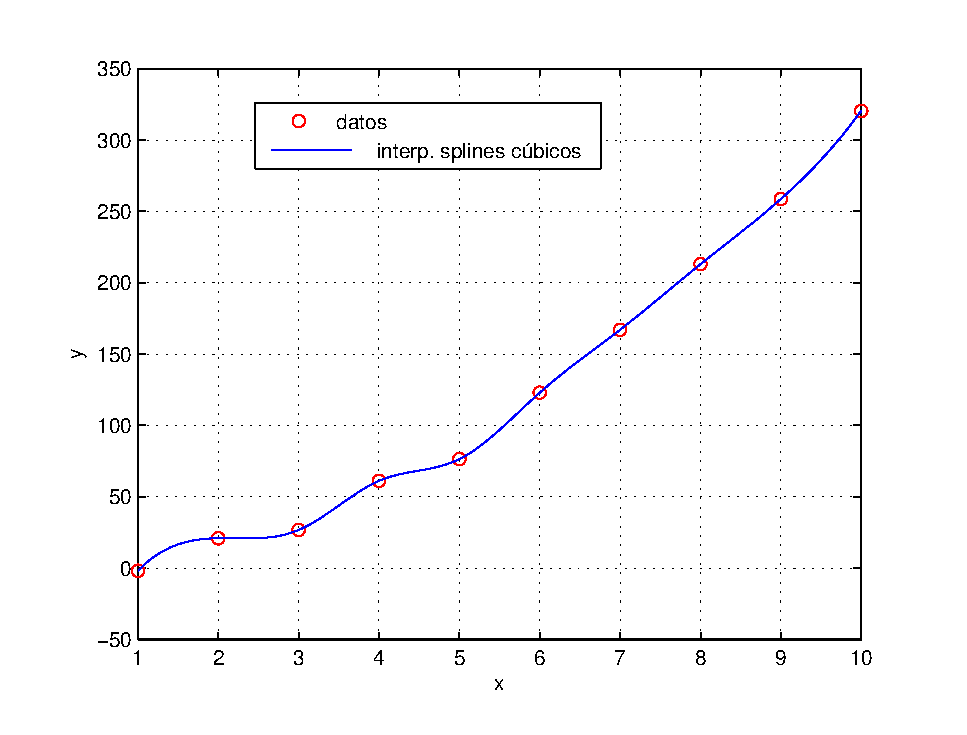
\includegraphics[width=12cm]{splines.eps}
	\bicaption{Interpolación mediante spline cúbico de los datos de la figura}{Cubic Spline interpolation for the data represented in the figure} \ref{fig:intepol} 
	\label{fig:splines}
\end{figure} 

\inputminted[
frame=lines,
framesep=2mm,
baselinestretch=1.2,
%bgcolor=LightGray,
label=ejemplo\_interp1d.py,
fontsize=\footnotesize,
linenos
]{python}{./codigos/interpolacion/ejemplo_interp1d.py}



\begin{paracol}{2}
La segunda función interpoladora de\\ \mintinline{python}{scipy.interpolation} que vamos a describir se llama \mintinline{python}{CubicSpline}. Permite interpolar empleando Splines cúbicos. En este caso, además de los datos $x$ e $y$ necesarios para definir el spline, la función admite el parametro \mintinline{python}{bc_type}, que permite determinar las condiciones de contorno en los extremos del spline. Las opciones posibles son: 

\mintinline{python}{bc_type='not__knot'}. Es la opcion por defecto. Hace que el polinomio empleado en el primer y segundo segmento en los extremos del spline sea el mismo.
 
\mintinline{python}{bc_type='natural'}. Spline natural.

\mintinline{python}{bc_type='periodic'}. Spline periódico.

Hay más opciones; los interesados pueden encontrarlas en la documentación de \mintinline{python}{scipy}. El uso es similar al descrito para \mintinline{python}{interp1d}. A partir de los datos se crea una función interpoladora que permite calcular el valor de la imagen en los puntos que se desee. Por ejemplo, para splines naturales sería,
\switchcolumn
 The second interpolating function, from\\ \mintinline{python}{scipy.interpolation} we are going to describe is \mintinline{python}{CubicSpline}. This function, as can be expected, uses cubic splines to perform the interpolation of a dataset. In this cases, in addition to the $x$ and $y$ data needed to define the spline, the function defines an input paramenter \mintinline{python}{bc_type}, which allows us to stablish the boundary conditions in the ends of the spline. Some of the available options are:
 
\mintinline{python}{bc_type='not__knot'}. This is the default option. The first and second segments at an end of the spline uses the same polynomial.

\mintinline{python}{bc_type='natural'}. Natural spline.

\mintinline{python}{bc_type='periodic'}. Periodic spline.

There are more options. Those interested can find them in \mintinline{python}{scipy} documentation. Its use  is similar to the use of \mintinline{python}{interp1d}. From the data we want to interpolate \mintinline{python}{CubiSpline} generates an interpoling function which alows us to compute the spline value in the point we wish. For instance, for natural splines we write, 
 
  
\end{paracol}
\begin{center}
\begin{minipage}{.5\textwidth}
\begin{minted}{python}
	spnat = CubicSpline(x,y,'natural')
	yi = spnat(xi)
\end{minted}
\end{minipage}
\end{center}

\begin{paracol}{2}
\section{Ajuste polinómico por el método de mínimos cuadrados}\label{sec:mc}\index{Mínimos cuadrados} \index{Ajuste polinómico}
\sectionmark{Mínimos cuadrados \textreferencemark\ Least squares}

Los métodos de interpolación que hemos descrito hasta ahora, pretenden encontrar un polinomio o una función definida a partir de polinomios que pase por un conjunto de datos. En el caso del ajuste por mínimos cuadrados, lo que se pretende es buscar el polinomio, de un grado dado, que mejor se aproxime a un conjunto de datos.

Supongamos que tenemos un conjunto de $m$ datos,
\switchcolumn
 \section{Least squared error me\-thod for polynomial data fitting}\index[eng]{Polinomial fitting}\index[eng]{Least Squared Error}
 
 The interpolation methods we have described so far, try to find a polynomial of a function defined using polynomials that passes through a set of data. In the case of Least squared error fitting, the aim is to find the polynomial of a specific degree that better approximates a dataset.
 
 Suppose we have a dataset holding $m$ data,        
\end{paracol}
\begin{table}[h]
\centering
\begin{tabular}{c|cccc}
x&$x_1$&$x_2$&$\cdots$&$x_m$\\
\hline
y&$y_1$&$y_2$&$\cdots$&$y_m$
\end{tabular}
\end{table} 
\begin{paracol}{2}
Queremos construir un polinomio $p(x)$  de grado $n < m-1$, de modo que los valores que toma el polinomio para los datos $p(x_i)$ sean lo más cercanos posibles a los correspondientes valores $y_i$. 

En primer lugar, necesitamos clarificar qué entendemos por \emph{lo más cercano posible}.  Una posibilidad, es medir la diferencia, $y_i-p(x_i)$ para cada par de datos del conjunto. Sin embargo, es más frecuente emplear el cuadrado de dicha diferencia, $\left(y_i-p(x_i)\right)^2$. Esta cantidad tiene, entre otras, la ventaja de que su valor es siempre positivo con  independencia de que la diferencia sea positiva o negativa. Además, representa el cuadrado de la distancia entre $p(x_i)$ e $y_i$. Podemos tomar la suma de dichas distancias al cuadrado, obtenidas por el polinomio para todos los pares de puntos, 
\switchcolumn
We want to build a polynomial $p(x)$ with degree $n < m-1$ so that the values it takes for the data $p(x_i)$ are the nearest possible to the values  $y_i$ of the data table.

First, we must clarify what means \emph{the nearest possible}. One option is to measure the difference $y_i -p(x_i)$ for each pair of data in the dataset. However, using the square of such difference  $\left(y_i-p(x_i)\right)^2$ is more common. This quantity has the advantage, among others, of being always positive, no matter whether the difference is positive or negative. Besides, it represents the square distance between $p(x_i)$ and $y_i$. We can take the sum of these differences for all pairs in the dataset,
\end{paracol}
\begin{equation*}
\sum_{i=1}^m \left(y_i-p(x_i)\right)^2
\end{equation*}
\begin{paracol}{2}
\noindent como una medida de la distancia del polinomio a los datos.  De este modo,  el polinomio \emph{lo más cercano posible}  a los datos sería aquel que minimice la suma de diferencias al cuadrado que acabamos de definir. De ahí el nombre del método.

En muchos casos, los datos a los que se pretende ajustar un polinomio por mínimos cuadrados son datos experimentales. En función del entorno experimental y del método con que se han adquirido los datos, puede resultar que algunos resulten más fiables que otros. En este caso, sería deseable hacer que el polinomio se aproxime más a los datos más fiables. Una forma de hacerlo es añadir unos \emph{pesos}, $\omega_i$, a las diferencias al  cuadrado en función de la confianza que nos merece cada dato,
\switchcolumn
\noindent as a measure of the distance from the polynomial to the data. In this way, the \emph{nearest possible to the data} would be the polynomial that minimised the sum of square differences we have just defined. Indeed, this is the origin of the method's name.

The data we often want to fit a polynomial using the least square method are experimental data. Depending on the environment and the method used for data acquisition, some data may be more reliable than others. In this case, it is interesting that the polynomial passes closest to the more reliable data. One way to achieve it is to add some \emph{weights}, $\omega_i$ to the square differences according to the confidence that each data deserves,    
\end{paracol}
\begin{equation*}
\sum_{i=1}^m \omega_i \left(y_i-p(x_i)\right)^2
\end{equation*}
\begin{paracol}{2}
Los datos fiables se multiplican por valores de $\omega$ grandes y los poco fiables por valores pequeños.

Para ver cómo obtener los coeficientes de un polinomio de mínimos cuadrados, empezaremos con el caso más sencillo; un polinomio de grado $0$. En este caso, el polinomio es una constante, definida por su término independiente $p(x)=a_0$. El objetivo a minimizar sería entonces,
\switchcolumn
We will multiply more reliable data by large values of $\omega$ and the less reliable by small values.

To see how to obtain the coefficients of a least square polynomial, we will start with the simplest case; a 0-degree polynomial. In this case the polynomial is a simple constant value, defined by its constant term $p(x) = a_0$. Then the fucntion to be minimised would be,
\end{paracol}
\begin{equation*}
g(a_0)=\sum_{i=1}^m \omega_i \left(y_i-a_0\right)^2
\end{equation*}
\begin{paracol}{2}
El valor mínimo de esta función debe cumplir que su derivada primera $g'(a_0)=0$ y que su derivada segunda  $g''(a_0)\geq 0$,
\switchcolumn
The minimum of this function must meet that its first derivative $g'(a_0)=0$ and its second derivative  $g''(a_0)\geq 0$,
\end{paracol}
\begin{align*}
g'(a_0)&=-2\sum_{i=1}^m \omega_i \left(y_i-a_0\right)=0 \Rightarrow a_0=\frac{\sum_{i=1}^m \omega_i\cdot y_i}{ \sum_{i=1}^m \omega_i}\\
g''(a_0)&=2\sum_{i=1}^m \omega_i \Rightarrow  g''(a_0) \geq 0
\end{align*}
\begin{paracol}{2}
El resultado obtenido para el valor de $a_0$ es una media, ponderada con los pesos $w_i$ de los datos. Si hacemos $w_i=1 \ \forall w_i$ obtendríamos exactamente la media de los datos. Este resultado resulta bastante razonable. Aproximar un conjunto de valores por un polinomio de grado cero, es tanto como suponer que la variable $y$ permanece constante para cualquier valor de $x$. Las diferencias observadas deberían deberse entonces a errores aleatorios experimentales, y la mejor estima del valor de $y$ será precisamente el valor medio de los valores disponibles. La figura \ref{fig:mc0} muestra el resultado de  calcular el polinomio de mínimos cuadrados de grado cero para un conjunto de datos.
\switchcolumn
We obtain that the value for $a_0$ is a mean of the data, weighted by the values $\omega_i$ assigned to the data. If we take  $w_i=1 \ \forall w_i$, we obtain the mean value of the data. This result is quite reasonable. Approximating a set of values with a 0-degree polynomial is equivalent to considering that variable $y$ remains constant for every value of $x$. In this case, we may attribute the observed differences among the values of the table to experimental random errors. Consequently, the best estimation of $y$ would be the mean value of the available data.       
\end{paracol}
\begin{figure}[h]
\centering
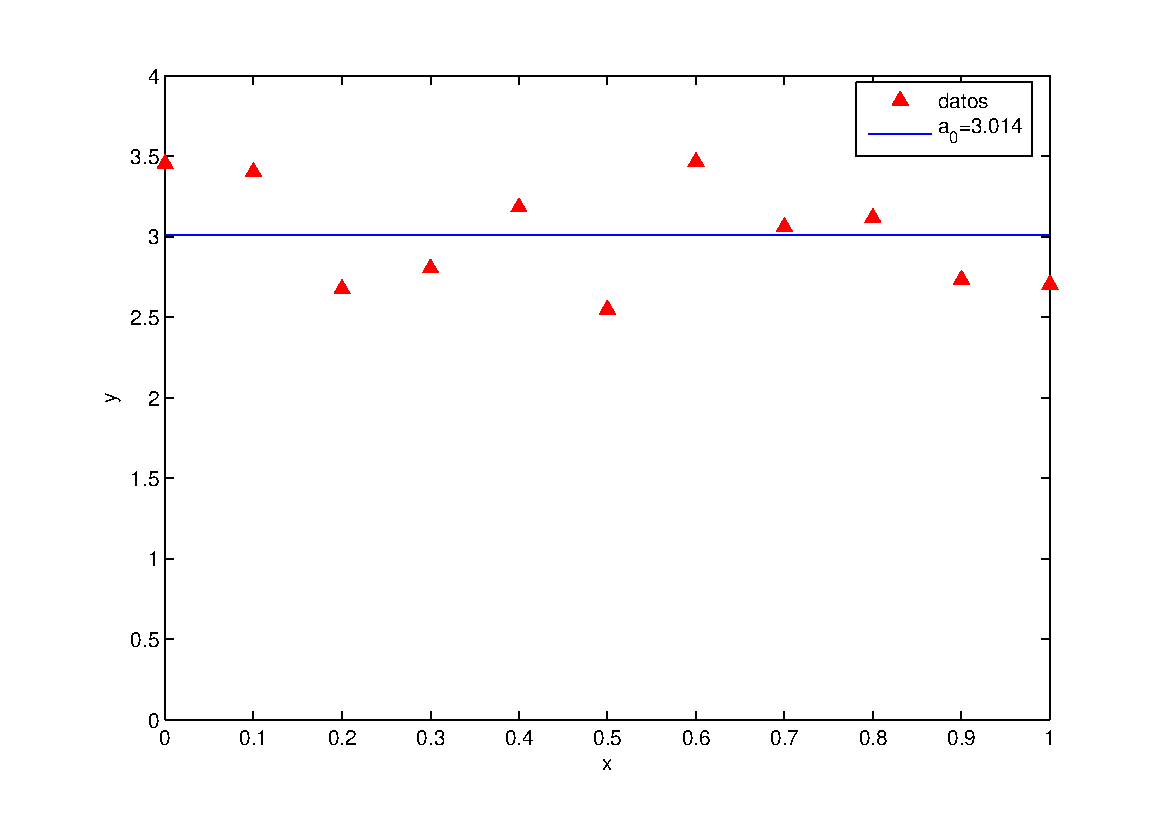
\includegraphics[width=12cm]{mc0.eps}
\bicaption{Polinomio de mínimos cuadrados de grado 0}{0-degree least squared error polynomial} 
\label{fig:mc0}
\end{figure} 
\begin{paracol}{2}
El siguiente paso en dificultad sería tratar de aproximar un conjunto de datos por un polinomio de grado 1, es decir, por una linea recta, $p(x)=a_0+a_1 x$. En este caso, la suma de diferencias al cuadrado toma la forma,
\switchcolumn The nest step would be to approximate the data using a 1-degree polynomial, i.e., a straight line, $p(x) = a_0+a_1x$. Inn this case, the sum of squared differences takes the form,
\end{paracol}
\begin{equation*}
g(a_0,a_1)=\sum_{i=1}^m \omega_i\left(y_i-a_0-a_1 x_i \right)^2
\end{equation*}
\begin{paracol}{2} 
En este caso, tenemos dos coeficientes sobre los que calcular el mínimo. Éste se obtiene cuando las derivadas parciales de $g(a_0,a_1)$ respecto a ambos coeficientes son iguales a cero.
\switchcolumn
We have now two coefficient for computing the minimum. We get the minimum making the function $g(a_0,a_1)$ partial derivatives equal to zero.   
\end{paracol}
\begin{align*}
\frac{\partial g}{\partial a_0}&=-2\sum_{i=1}^m \omega_i (y_i-a_0-a_1 x_i) = 0\\
\frac{\partial g}{\partial a_1}&=-2\sum_{i=1}^m \omega_i x_i(y_i-a_0-a_1 x_i) = 0
\end{align*} 
\begin{paracol}{2}
Si reordenamos las ecuaciones anteriores,
\switchcolumn
And after rearranging the previous equations,
\end{paracol}
\begin{align*}
&\left(\sum_{i=1}^m \omega_i\right)a_0+ \left(\sum_{i=1}^m \omega_ix_i\right)a_1 =\sum_{i=1}^m \omega_iy_i\\
&\left(\sum_{i=1}^m \omega_ix_i\right)a_0+ \left(\sum_{i=1}^m \omega_ix_i^2\right)a_1 =\sum_{i=1}^m \omega_ix_iy_i
\end{align*}
\begin{paracol}{2}
Obtenemos un sistema de dos ecuaciones lineales cuyas incógnitas son precisamente los coeficientes de la recta de mínimos cuadrados.

Podemos ahora generalizar el resultado para un polinomio de grado $n$, $p(x)=a_0+a_1x+a_2x^2+\cdots +a_nx^n$. La función $g$ toma la forma,

\switchcolumn
We get a linear system with two equations and two unknowns, which are the coefficients of the least squares line.

We can now generalised this result for a $n$-degree polynomial $p(x)=a_0+a_1x+a_2x^2+\cdots +a_nx^n$. Function $g$ would be now,
\end{paracol}
\begin{equation*}
g(a_0,a_1,\cdots, a_n)=\sum_{i=1}^m \omega_i \left (a_0+a_1x_i+\cdots+ a_nx_i^n-y_i\right)^2
\end{equation*}
\begin{paracol}{2}
De nuevo, para obtener los coeficientes del polinomio igualamos las derivadas parciales a cero,
\switchcolumn
Again, we can get the polynomial coefficents making the partial derivatives equal to zero,
\end{paracol}
\begin{equation*}
\frac{\partial g(a_0,a_1,\cdots, a_n)}{\partial a_j}=0 \Rightarrow \sum_{i=1}^m \omega_i x_i^j \left( a_0+a_1x_i+\cdots + a_nx_i^n-y_i\right)=0, \ j=0,1\cdots, n
\end{equation*} 
\begin{paracol}{2}
Si reordenamos las expresiones anteriores, llegamos a un sistema de $n+1$ ecuaciones lineales, cuyas incógnitas son los coeficientes del polinomio de mínimos cuadrados,
\switchcolumn
If we rearrange the previous equation, we arrive to a linear system of $n+1$ equations whose unknowns are the coefficients of the least squares polynomial,
\end{paracol}
\begin{equation*}
\begin{pmatrix}
s_0& s_1& \cdots s_n\\
s_1& s_2& \cdots s_{n+1}\\
\vdots & \vdots & \ddots \\
s_n& s_{n+1}& \cdots s_{2n}\\
\end{pmatrix}\cdot \begin{pmatrix}
a_0\\
a_1\\
\vdots \\
a_n
\end{pmatrix}=\begin{pmatrix}
c_0\\
c_1\\
\vdots \\
c_n
\end{pmatrix}
\end{equation*} 
\begin{paracol}{2}
Donde hemos definido $s_j$ y $c_j$ como,
\switchcolumn
Where we have defined $s_j$ and $c_j$ as,
\end{paracol}
\begin{align*}
s_j&=\sum_{i=1}^m \omega_ix_i^j\\
c_j&=\sum_{i=1}^m \omega_ix_i^jy_i
\end{align*}
\begin{paracol}{2} 
El siguiente código permite obtener el polinomio de mínimos cuadrados que aproxima un conjunto de $n$ datos,
\switchcolumn
h following code calculates the coefficients of the least squares polynomial that approximate a set of $n$ data.
\end{paracol}
\inputminted[
frame=lines,
framesep=2mm,
baselinestretch=1.2,
%bgcolor=LightGray,
label=minimos\_cuadrados.py,
fontsize=\footnotesize,
linenos
]{python}{./codigos/interpolacion/minimos_cuadrados.py}


\begin{paracol}{2}
Una última observación importante es que si intentamos calcular el polinomio de mínimos cuadrados de grado $m-1$ que aproxima un conjunto de $m$ datos, lo que obtendremos será el polinomio de interpolación. En general, cuanto mayor sea el grado del polinomio más posibilidades hay de que la matriz de sistema empleado para obtener los coeficientes del polinomio esté mal condicionada.

\subsection{Mínimos cuadrados en Py\-thon.}

Hay varias formas de llevar a cabo un ajuste polinómico por mínimos cuadrados empleando Python. Solo vamos a describir uno de ellos. El subpaquete de \mintinline{python}{numpy}, \mintinline{python}{numpy.polynomial} incluye una clase llamada \mintinline{python}{Polynomial} (con mayúscula) permite, entre otras cosas, crear polinomios como objetos de programación. Una de las formas de crear un polinomio, es como resultado del ajuste por mínimos cuadrados a un conjunto de datos. Para ello, \mintinline{python}{Polynomial}, cuenta con la función \mintinline{python}{fit}. Este comando admite como entradas un vector de coordenadas $x$ y otro de coordenadas $y$, de los datos que se quieren aproximar, y una tercera variable con el grado del polinomio. Opcionalmente se puede añadir un vector de pesos, si se quiere ponderar la importancia que damos a cada dato. 

La funcion \mintinline{python}{Polynomial.fit} devuelve como resultado un 'objeto' polinomio. Este objeto contiene toda la información sobre el polinomio creado y puede usarse directamente como una función para calcular el valor del polinomio en un punto. El siguiente script de Python crea un par de vectores y muestra como manejar el comando,
\switchcolumn
A last important remark: If we try to compute the least squared error polynomial of degree $m-1$ to approximate a set of $m$ data, we will get the interpolating polynomial. In general, if we increase the degree of the least squared polynomial, we increase the probability that the system matrix we use to obtain the polynomial coefficients will be poorly conditioned.

\subsection{Least squares in Python.}
There are several ways to compute the Le\-ast squares polynomial for a set of data using Py\-thon. We will describe only one of them. The \mintinline{python}{numpy} sub-package \mintinline{python}{numpy.polynomial} includes a class called \mintinline{python}{Polynomial} (Mean the first capital letter!) allows us, among many other things, to create polynomial as programming objects. One way to create a polynomial is to compute the least squares polynomial from a dataset. The class \mintinline{python}{Polynomial} has a special function \mintinline{python}{fit} to accomplish it. This command takes as inputs two arrays of data, one with the coordinates $x$ and the other with the coordinates $y$ of the value we want to interpolate, plus a third variable for the polynomial degree. Optionally, we can add an array of weights to balance the importance we give to each data.

Function \mintinline{python}{Polynomial.fit} returns a polynomial 'object'. This object contains all the information on the polynomial it represents and it can be use straightforwardly as a function to compute the value of the polynomial in any point. The following Python's script generates a pair of vectors and shows how to deal with the \mintinline{python}{fit} command. 
\end{paracol}

\inputminted[
frame=lines,
framesep=2mm,
baselinestretch=1.2,
%bgcolor=LightGray,
label=ejemplo\_ajuste.py,
fontsize=\footnotesize,
linenos
]{python}{./codigos/interpolacion/ejemplo_ajuste.py}

\begin{paracol}{2}
Vamos a revisar algunos puntos importantes de este código. en la línea 8, importamos el objeto \mintinline{python}{Polynomial}. Lo hacemos siguiendo el mismo método con que habríamos importado un submódulo cualquiera de \mintinline{python}{numpy}. Le asignamos el alias \mintinline{python}{py}.
En la línea 12 hemos importado la función lse. Se trata de la función que hemos creado nosotros para realizar ajustes por mínimos cuadrados y cuyo código hemos incluido mas arriba. En las líneas 15 y 16 creamos un conjunto de datos.

En la línea 20 creamos un polinomio de minimos cuadrados de grado 3, \mintinline{python}{p3}, que ajusta los datos anteriores. \mintinline{python}{p3}, contiene toda la información del polynomio creado. En la línea 22, empleamos el comando \mintinline{python}{convert} para obtener un array con los coeficientes del polinomio, ordenados de menor a mayor grado. $p(x)=a_0 + a_1x +a_2x^2+\cdots+a_nx^n$. En la línea 27 empleamos directamente \mintinline{python}{p3} como una función, pasándole los valores del array \mintinline{python}{xi}, para evaluar el polinomio en dichos puntos.

En las líneas 29-34 repetimos el cálculo, pero ahora empleando pesos. Damos a todos los pesos un valor $1$ excepto para el quinto dato, al que damos un peso menor.

Las líneas 39 a 45 repiten los mismos cálculos, pero ahora empleando la función \mintinline{python}{lse}, creada por nosotros.

Por último, dibujamos los resultados para compararlos, tal y como se muestran en la figura \ref{fig:lse}
\switchcolumn
We are going to review some important points of the previous code. In line 8, we import the object \mintinline{python}{Polynomial}. We do it in the same way that we import whatever \mintinline{python}{numpy} submodule. We have assigned to \mintinline{python}{Polynomial} the alias \mintinline{python}{py}. In line 12 we import the function \mintinline{python}{lse}. This is the function we previously created to perform least squares fits and whose code we included above. In lines 15 and 16 we create a dataset.

In line 20, we create a 3-degree least squares polynomial, \mintinline{python}{p3}, which fits the previous data. \mintinline{python}{p3} holds all the information on the polynomial we have created. In line 22, we use the command \mintinline{python}{convert} to obtain an array with the polynomial coefficients, ordered in ascending degree. $p(x)=a_0 + a_1x +a_2x^2+\cdots+a_nx^n$. In line 27, we use \mintinline{python}{p3} straightforwardly, as a function, to obtain the values the polynomial takes at the points held by the array \mintinline{python}{x_i}.

We repeat the same computation in lines 29-34 but now use weights. We assign a value of $1$ to every weight except for the fifth data point, to which we assign a smaller weight.

In lines 39 to 45 we repeat the the same computation but this time using our own function, \mintinline{python}{lse}

Lastly, we draw the results to compare, as can be seen in figure \ref{fig:lse}.
\end{paracol}

\begin{figure}[h]
	\centering
	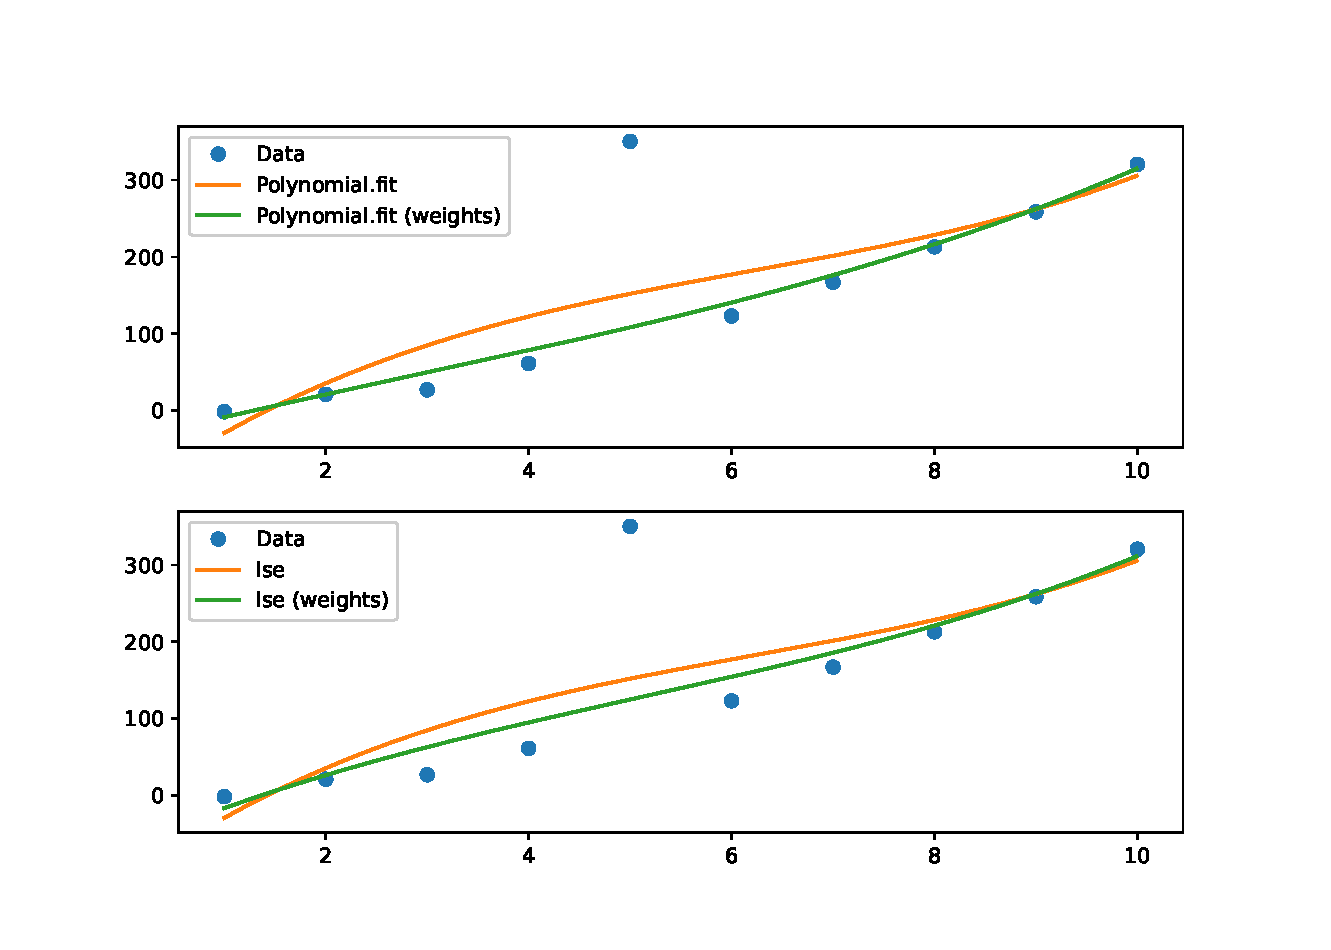
\includegraphics[width=0.9\textwidth]{ejemplo_lse.eps}
	\bicaption{Ejemplo de cálculo de ajuste por mínimos cuadrados empleando la función fit de Polynomial y nuestra función lse.}{An example of least squares polynomial fit, using the function fit from Polynomial and our function lse.}
	\label{fig:lse}
\end{figure}


\begin{paracol}{2}
La figura muestra claramente el efecto de los pesos en la regresión. Al atenuar la influencia del quinto punto, que claramente parece fuera de rango, la curva se acerca más al resto de los puntos.

Si miramos con atención ambos gráficos, es fácil darse cuenta que la función de Python acerca más el polinomio a los puntos que la que hemos escrito nosotros. La razón está en que hemos usado un modo distinto de introducir los pesos. La función \mintinline{python}{fit}, aplica el el peso directamente a la diferencia entre el dato y el valor del polinomio $\omega_i \vert y_i - p(x_i)\vert$ mientras que nosotros aplicamos los pesos al cuadrado de dicha diferencia $\omega_i(y_i-p(x_i))^2$. Si comparamos lo coeficientes de los polinomios obtenidos,

\switchcolumn
The figure clearly shows the effect the we\-ights have on the regression results. When we attenuate the influence of the fifth point, which appears to be quite an outlier, the curve approaches more to the remaining points.

If we look at both graphics attentively, we will see that the Python function approximates the polynomial more to the points than the function we have written. The difference comes from how we introduce the weights, which are not the same as those used by Python. Function \mintinline{python}{fit}, applies the weights directly to the difference between the data an the value taken by the polynomial $\omega_i \vert y_i - p(x_i)\vert$, whike our function applies the weights to the squared difference  $\omega_i(y_i-p(x_i))^2$. If we compare the coefficients of the polynomials computed by both methods,
\end{paracol}

\begin{minted}{python}
In [47]: p3w.convert().coef
Out[47]: array([-40.71774313,  33.22583298,  -1.61930914,   0.1854822 ])
	
In [48]: aw
Out[48]: array([-68.26797522,  56.50545799,  -5.31193931,   0.34603134])
\end{minted}

\begin{paracol}{2}
vemos que no coinciden. Para obtener el mismo resultado, deberíamos introducir el cuadrado del valor de los pesos cuando usamos nuestra funcion,
\switchcolumn
We can see they are different. To get the same result, we must introduce the squared values of our weight when we use our function,

\end{paracol}
\begin{minted}{python}
In [49]: aw2 = lse(x,y,3,w**2)

In [50]: aw2
Out[50]: array([-40.71774313,  33.22583298,  -1.61930914,   0.1854822 ])
\end{minted}

\begin{paracol}{2}
Esto nos enseña una lección muy importante: no se deben emplear nunca paquetes de cálculo numérico sin saber qué están calculando exactamente. 	
\subsection{Análisis de la bondad de un ajuste por mínimos cuadrados.} \index{Mínimos cuadrados! Residuos}
Supongamos que tenemos un conjunto de datos obtenidos como resultado de un experimento. En muchos casos la finalidad de un ajuste por mínimos cuadrados, es encontrar una ley que nos permita relacionar los datos de la variable independiente con la variable dependiente. Por ejemplo si aplicamos distintas fuerzas a un muelle y medimos la elongación sufrida por el muelle, esperamos obtener, en primera aproximación, una relación lineal: $\Delta x\propto F$. (Ley de Hooke). 

Sin embargo, los resultados de un experimento rara vez se ajustan a una ley debido a errores aleatorios que no es posible corregir.

Cuando realizamos un ajuste por mínimos cuadrados de $m$ datos, podemos emplear cualquier polinomio desde grado $0$ hasta grado $m-1$. Desde el punto de vista del error cometido con respecto a los datos disponibles el mejor polinomio sería precisamente el de grado $m-1$ que da error cero para todos los datos, por tratarse del polinomio de interpolación. Sin embargo, si los datos son experimentales estamos incluyendo los errores experimentales en el ajuste.

Por ello, para datos experimentales y suponiendo que los datos solo contienen errores aleatorios, el mejor ajuste lo dará el polinomio de menor grado para el cual las diferencias entre los datos y el polinomio $y_i-p(x_i)$ se distribuyan aleatoriamente. Estas diferencias reciben habitualmente el nombre de residuos. \index{Residuos} 

\switchcolumn
This result teaches us a fundamental lesson: never use a numerical computing software package without understanding its operations.

\subsection{Analyzing goodness of fit using least squares method.}
Suppose we have a dataset we have obtained as a result of an experiment. In many cases, least squares data fitting aims to find a law that allows us to establish a mathematical relationship between the independent and dependent variables. For instance, if we apply different stresses to a spring and measure the elongation acquired by the spring, we expect to get a linear relationship between stress and elongation as a first approximation: $\Delta x\propto F$. (Hooke's law).

However, the results of an experiment hardly ever fit precisely into any law due to random errors, which we cannot amend.

When we carry out a least squares fitting, we may use any polynomial of degrees 0 to $m-1$. From the point of view of the error we make, considering only the available data, the best polynomial would be the $m-1$-degree polynomial because this is the interpolation polynomial, and, so, it makes a zero error for every data. Nevertheless, if we are trying to fit experimental data, we are including the experimental errors in the fitting.

As a consequence, for experimental data and assuming that the data only are affected by random errors, we get the best fitting using the polynomial of lest degree for which the differences between data and polynomial value $y_i-p(x_i)$ are randomly distributed. Such differences are usually called residuals. \index[eng]{residuals}
\end{paracol}

\begin{figure}
	\centering
	\subfigure[Recta de mínimos cuadrados y residuos obtenidos / Least squares line and residuals.  \label{fig:residuos1}]{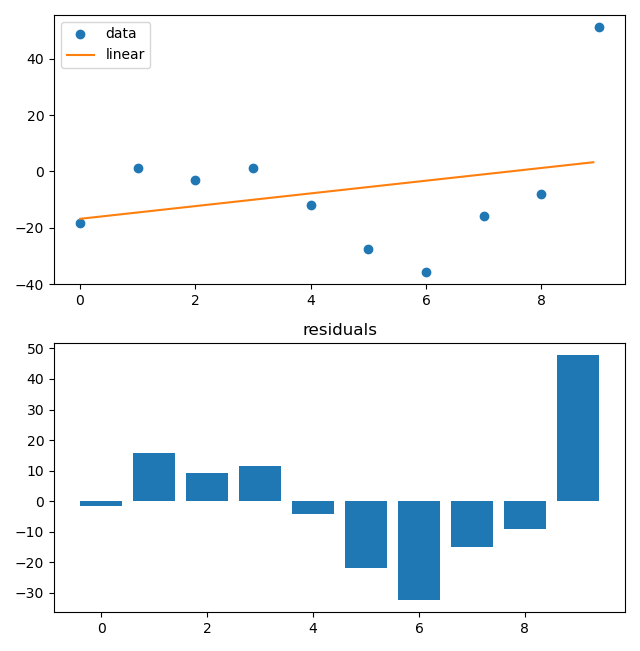
\includegraphics[width=7cm]{lse1.png}} \qquad 
	\subfigure[Parabola de mínimos cuadrados y residuos obtenidos / Least squares parabola and residuals.  \label{fig:residuos2}]{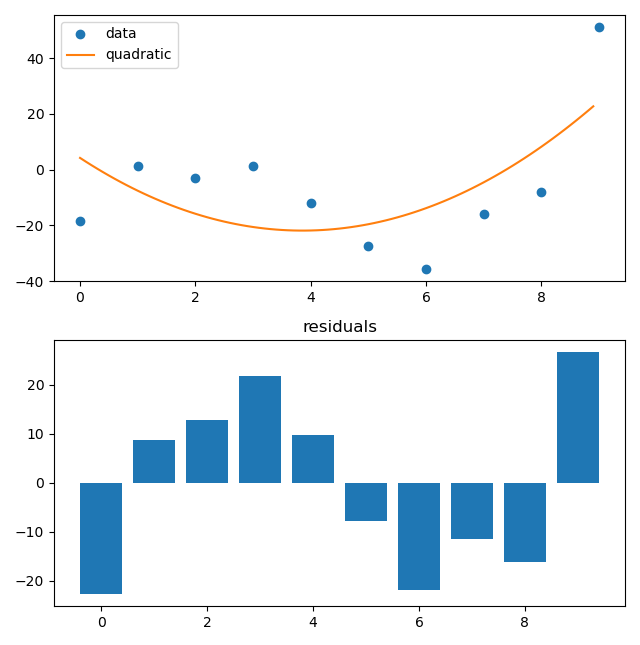
\includegraphics[width=7cm]{lse2.png}}\\
	\subfigure[polinomio de tercer grado  de mínimos cuadrados y residuos obtenidos / 3-degree polynomial and residuals  \label{fig:residuos3}]{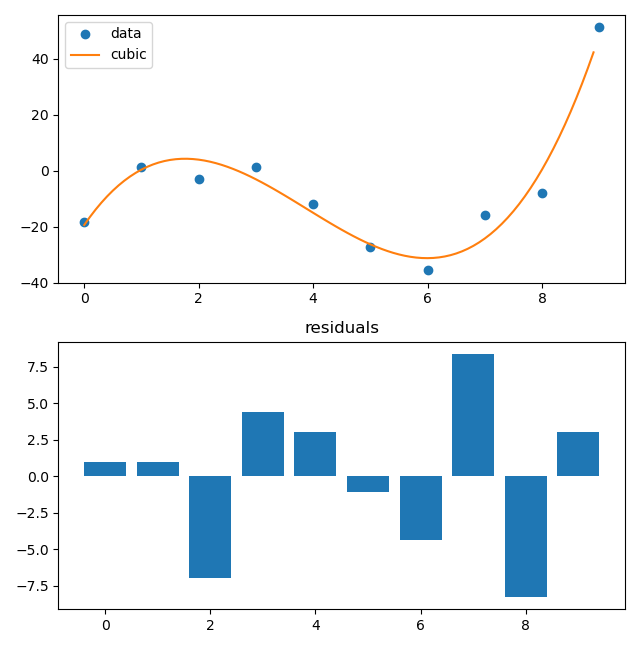
\includegraphics[width=7cm]{lse3.png}} \qquad 
	\subfigure[polinomio de cuarto grado  de mínimos cuadrados y residuos obtenidos / 4-degree polynomial and residuals \label{fig:residuos4}]{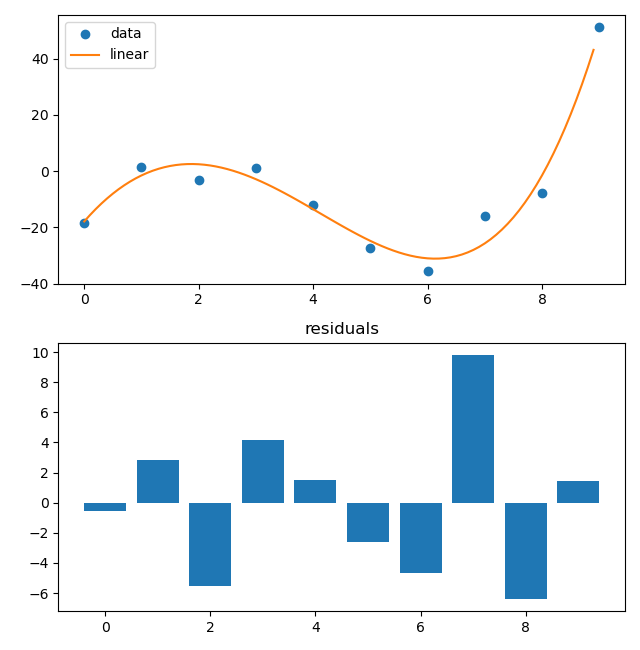
\includegraphics[width=7cm]{lse4.png}}
	\bicaption{Comparación entre los residuos obtenidos para los ajustes de mínimos cuadrados de un conjunto de datos empleando polinomios de grados 1 a 4.}{Comparison among the residuals resulting from a dataset least squares fitting, using polynomials of degrees 1 to 4.} 
	\label{fig:residuos}
\end{figure}
\begin{paracol}{2}
La figura \ref{fig:residuos} muestra un ejemplo de ajuste por mínimos cuadrados empleando cada vez un polinomio de mayor grado.
    
En la figura \ref{fig:residuos1} se observa claramente que el ajusto no es bueno, la recta de mínimos cuadrados no es capaz de adaptarse a la forma que presentan los datos. Los residuos muestran claramente esta tendencia: no están distribuidos de forma aleatoria. En la figura \ref{fig:residuos2}, la parábola aproxima mejor el conjunto de datos. Sin embargo, los residuos presentan un máximo y un mínimo suaves, no son realmente aleatorio. En la figura \ref{fig:residuos3}, los residuos están distribuidos de forma aleatoria. Si comparamos estos resultados con los de la figura \ref{fig:residuos4} vemos que en este último caso los residuos son más pequeños, pero conservan esencialmente la misma distribución aleatoria que en la figura anterior. La aproximación de los datos empleando un polinomio de cuarto grado no añade información sobre la forma de la función que siguen los datos, y ha empezado a incluir en el ajuste los errores de los datos.
\switchcolumn
Figure \ref{fig:residuos} shows a least square fitting  example, using polynomials of increasing degrees.  

The residual also shows the data shape; they are not randomly distributed. In figure \ref{fig:residuos2}, we can see how a parabola better approximates the data but cannot follow the data up and down. The residuals clearly show a smooth maximum and minimum, but they are not actually random. In figure \ref{fig:residuos3}, the polynomial fits better the data, and the residuals are randomly distributed. If we compare them with the residuals presented in figure \ref{fig:residuos4}, we see these last are smaller but present essentially the same random distribution. We may conclude that the data approximation using a fourth-degree polynomial does not add any useful information on the function shape the data follow, and, worse than this, we are starting to include the data errors in the fitting.
\end{paracol}
\begin{flalign*}
	&\mathwitch*_{i=0}^{\infty}\Xi_i(t) \Biggl \{&     
\end{flalign*}
\begin{paracol}{2}
\section{Curvas de Bézier}\index{Bézier}\index{Curvas de Bézier}
\sectionmark{Curvas de Bézier \textreferencemark\ Bézier's curves}
Las curvas de Bézier permiten unir puntos mediante curvas de forma arbitraria.  Una curva de Bézier viene definida por un conjunto de $n+1$ puntos, $\left\lbrace\vec{p}_0, \vec{p}_2, \cdots, \vec{p}_n\right\rbrace$, que reciben el nombre de puntos de control. El orden en que se presentan los puntos de control es importante para la definición de la curva de Bézier correspondiente. Ésta pasa siempre por los puntos $\vec{p_0}$ y $\vec{p_n}$. El resto de los puntos de control permiten dar forma a la curva, que tiene siempre la propiedad de ser tangente en el punto $\vec{p}_0$ a la recta que une $\vec{p}_0$ con $\vec{p}_1$ y tangente en el punto $\vec{p}_n$ a la recta que une $\vec{p}_{n-1}$ con $\vec{p}_n$.

Para definir la curva, se asocia a cada punto de control $\vec{p}_i$ una función conocida con el nombre de función de fusión. En el caso de las curvas de Bézier, las funciones de fusión empleadas son los polinomios de Bernstein, \index{Polinomios de Bernstein}
\switchcolumn	
\section{Bézier Curves} \index[eng]{Bézier}\index[eng]{Bézier's curves}
Bezier's curves can connect points using curves with arbitrary shape. We define a Bezier's curve using a set of of $n+1$ points, $\left\lbrace\vec{p}_0, \vec{p}_2, \cdots, \vec{p}_n\right\rbrace$ which are known as control points. The order of the control points play a key role in the definition of the corresponding Bézier's curve. The curve pass through the end points $\vec{p}_0$ and $\vec{p}_n$. The remaining control points allow us to define the curve shape, which has the interesting properties of being always tangent in point $\vec{p}_0$ to the line that connects $\vec{p}_0$ with $\vec{p}_1$ and tangent in point $\vec{p}_n$ to the line that connect $\vec{p}_{n-1}$ with $\vec{p}_n$.

 To define the curve, we associate to the control point $\vec{p}_i$, a function known as fusion function. In the case of Bezier's curves, we use as fusion function Berstein's polynomials,   
\end{paracol}
\begin{equation*}
B_i^n (t)=\binom{n}{i}\left(1-t\right)^{n-i}t^i, \quad i = 0, 1, \dots, n
\end{equation*}
\begin{paracol}{2}
El grado de los polinomios de Bernstein empleados depende del número de puntos de control; para un conjunto de $n+1$ puntos, los polinomios son de grado $n$. La variable $t$ es un parámetro que varía entre $0$ y $1$.

La ecuación de la curva de Bézier que utiliza un conjunto de $n+1$ puntos de control, $\left\lbrace\vec{p}_0, \vec{p}_2, \cdots, \vec{p}_n\right\rbrace$, se define a partir de los polinomios de Bernstein como,
\switchcolumn
The Berstein's polynomials degree we use depends on the number of control points; for a set of $n+1$, we need polynomials of degree $n$. Variable $t$ is a parameter which varies between 0 and 1.

The Bezier's curve for a set of $n+1$ control points,  $\left\lbrace\vec{p}_0, \vec{p}_2, \cdots, \vec{p}_n\right\rbrace$, can be defined using Berstein's polynomials, according to the following equation,  
\end{paracol}
\begin{equation*}
\vec{p}(t) = \sum_{i = 0}^n B_i^n(t) \cdot \vec{p}_i = \sum_{i = 0}^n \binom{n}{i}\left(1-t\right)^{n-i}t^i  \cdot \vec{p}_i
\end{equation*}
\begin{paracol}{2}
La expresión anterior da como resultado $\vec{p}_0$ si hacemos $t = 0$ y $\vec{p}_n$ si hacemos $t = 1$. para los valores comprendidos entre $t=0$ y $t=1$, los puntos $\vec{p}(t)$  trazarán una curva entre $\vec{p}_0$  y $\vec{p}_n$.

Veamos un ejemplo sencillo. Supongamos que queremos unir los puntos $\vec{p}_0 = (0,1)$ y $\vec{p}_n = (3,1)$ mediante curvas de Bézier. Si no añadimos ningún punto más de control, $\lbrace\vec{p}_0 = (0,1), \vec{p}_1 = (3,1)\rbrace$, la curva de Bézier que obtendremos será una recta que unirá los dos puntos,

\switchcolumn
The above expression yields $\vec{p}_0$ as a result, if we take $t=0$ and $\vec{p}_n$ for $t=1$. For values of $t$ between $t=0$ and $t=1$, points $\vec{p}(t)$ will describe a curve between $\vec{p}_0$  y $\vec{p}_n$.  

Let's see a basic example. Suppose we want to connect point $\vec{p}_0 = (0,1)$ with point $\vec{p}_1$ using a Bezier's curve. If we do not define any other control point, $\lbrace\vec{p}_0 = (0,1), \vec{p}_1 = (3,1)\rbrace$, The Bezier's curve we will obtain will be a line connection both points.
\end{paracol}
\begin{equation*}
\vec{p}(t) = \binom{1}{0}\left(1-t\right)^{1}t^0  \cdot (0,1) +  \binom{1}{1}\left(1-t\right)^{0}t^1  \cdot (3,1) = \left(1-t\right)  \cdot (0,1) + t\cdot (3,1)
\end{equation*} 
\begin{paracol}{2}
Si separamos las componentes $x$ e $y$ del vector $\vec{p}(t)$,

\switchcolumn
If we split the components $x$ and $y$ of vector $\vec{p}(t)$,
\end{paracol}

\begin{align*}
x &= 3t\\
y &= 1
\end{align*}
\begin{paracol}{2}
Se trata de la ecuación del segmento horizontal que une los puntos $\vec{p}_0 = (0,1)$ y $\vec{p}_n = (3,1)$ 

Si añadimos un punto más de control, por ejemplo:  $\vec{p}_1 = (1,2) \rightarrow \lbrace\vec{p}_0 = (0,1), \vec{p}_1 = (1,2), \vec{p}_2 = (3,1)\rbrace$,  la curva resultante será ahora un segmento de un polinomio de segundo grado en la variable $t$,
\switchcolumn
It is the equation of the horizontal segment that joints the points $\vec{p}_0 = (0,1)$ y $\vec{p}_n = (3,1)$

If we add a control point more, for instance:  $\vec{p}_1 = (1,2) \rightarrow \lbrace\vec{p}_0 = (0,1), \vec{p}_1 = (1,2), \vec{p}_2 = (3,1)\rbrace$, the resulting curve will be now a segment of a second degree polynomial on the variable $t$,
\end{paracol}
\begin{align*}
\vec{p}(t) &= \binom{2}{0}\left(1-t\right)^{2}t^0  \cdot (0,1) +  \binom{2}{1}\left(1-t\right)t \cdot (1,2) + \binom{2}{2}\left(1-t\right)^{0}t^2  \cdot (3,1) =\\
&= \left(1-t\right)^{2} \cdot (0,1) + 2 \left(1-t\right)t \cdot (1,2) + t^2  \cdot (3,1) 
\end{align*} 
\begin{paracol}{2}
Según vamos aumentando el número de los puntos de control, iremos empleando polinomios de mayor grado. El segmento de polinomio empleado en cada caso para unir los puntos de control inicial y final variará dependiendo de los puntos de control intermedios empleados.

La figura \ref{fig:bezier} muestra un ejemplo en el que se han construido varias curvas de Bézier sobre los mismos puntos de paso inicial y final. Es fácil observar cómo la forma de la curva depende del número y la posición de los puntos de control. Si unimos éstos por orden mediante segmentos rectos, obtenemos un polígono que recibe el nombre de polígono de control. En la figura \ref{fig:bezier} se han representado los polígonos de control mediante líneas de puntos.

El siguiente código permite calcular y dibujar una curva de Bézier a partir de sus puntos de control, empleando las funciones \mintinline{python}{bezier} y \mintinline{python}{bezier_sc}
\switchcolumn
As we increase the number of control points, we also increase de degree of the polynomial used to connect the first and last control points. The shape of this polynomial will change depending on the intermediate control point we use. 

Figure \ref{fig:bezier} shows an example in which we have built several Bézier's curves using the same initial and final controls points. Notice how the shape of the curve depends on the number and position of the control points. If we orderly connect the control points using straight segments we get a polygon know as control polygon. In figure \ref{fig:bezier} the control polygons have been represented using dashed lines.

The following code includes functions  \mintinline{python}{bezier} and \mintinline{python}{bezier_sc} to compute and draw Bezier's curves define from their control points.
\end{paracol}

\begin{figure}
\centering
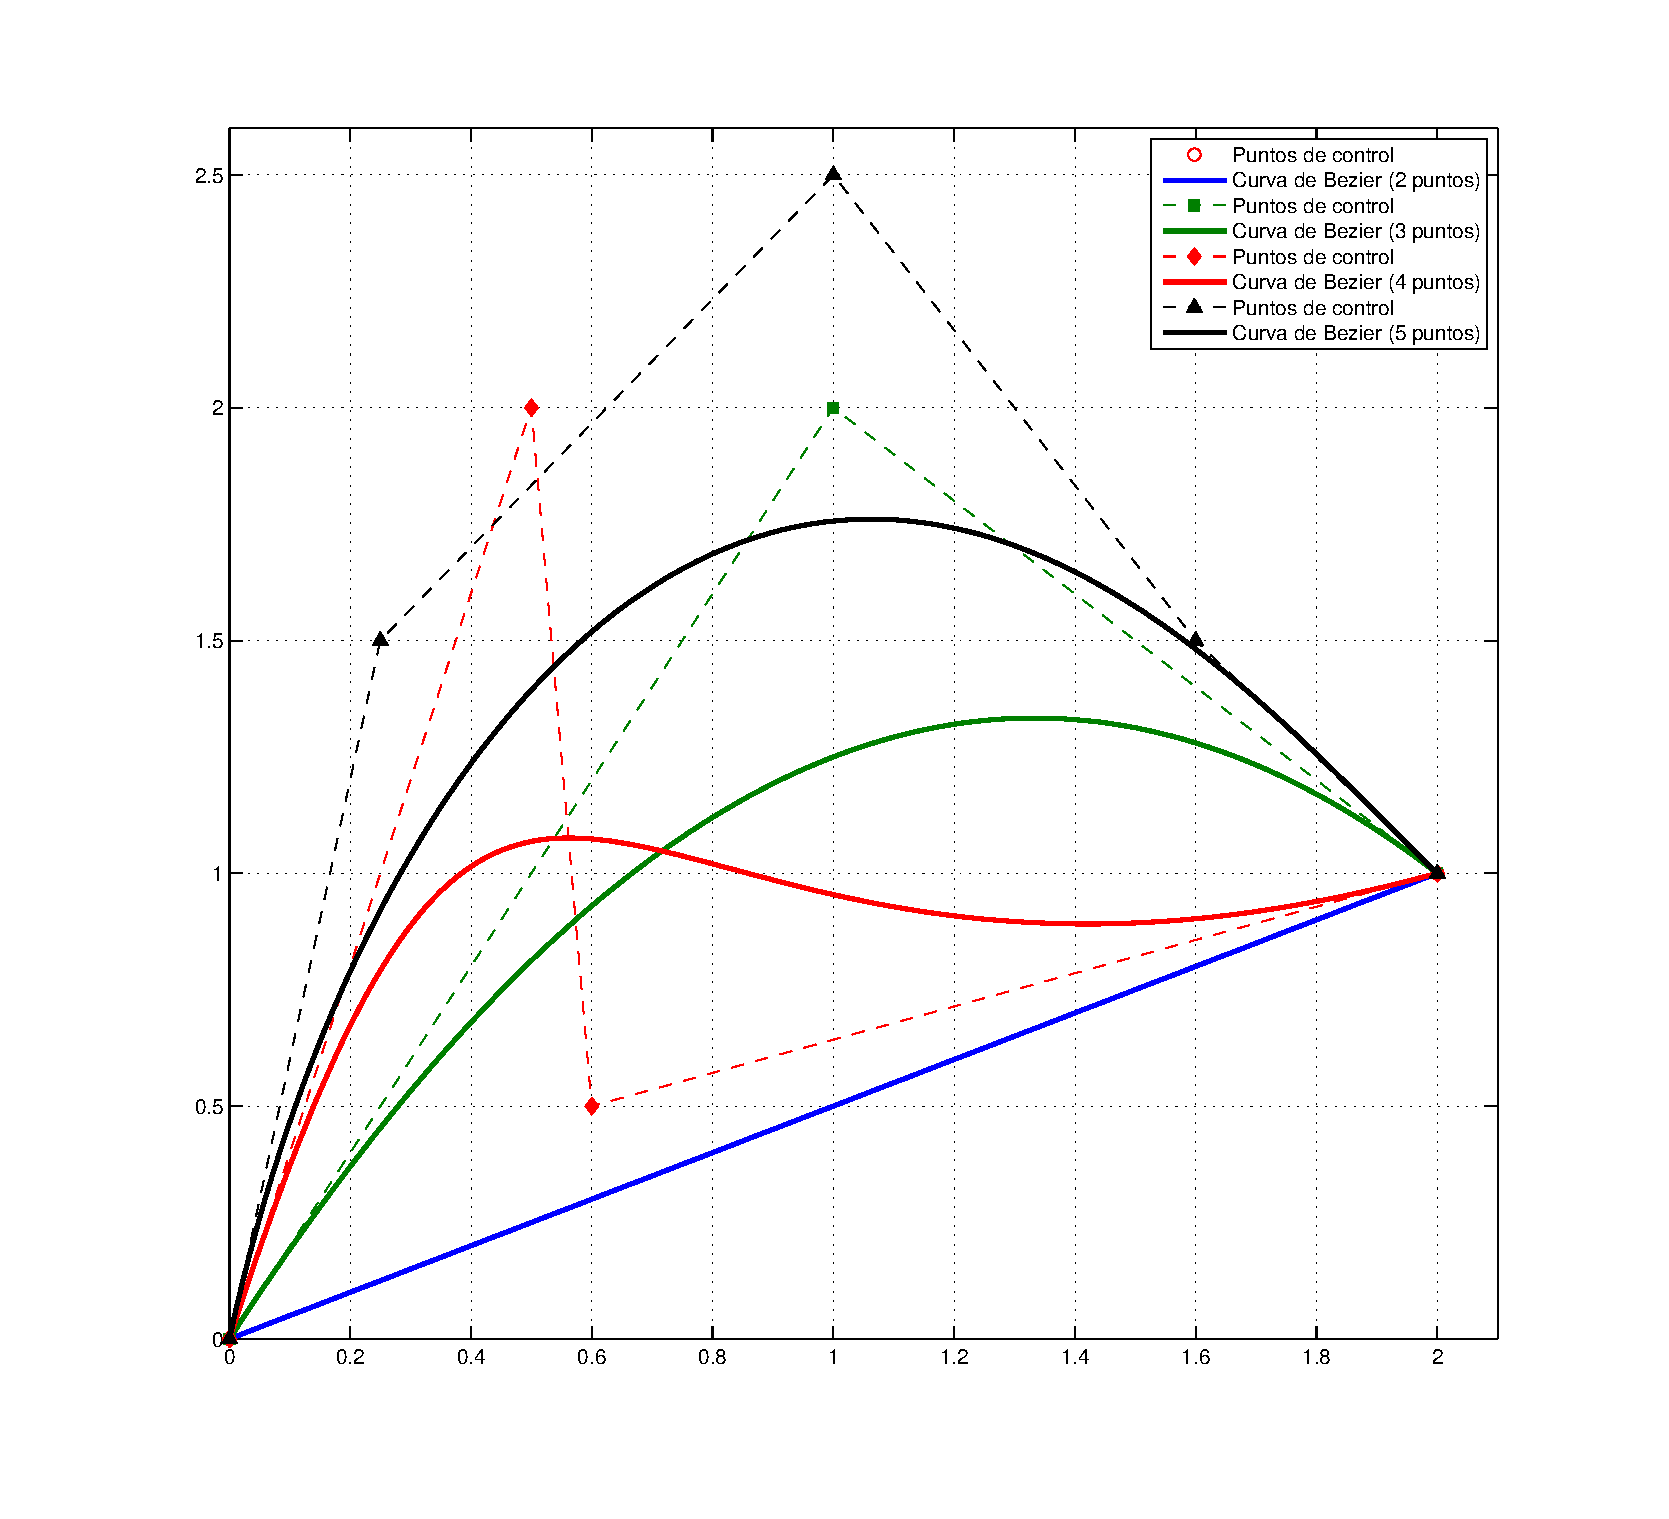
\includegraphics[width=10cm]{bezier.eps} 
\bicaption{Curvas de Bézier trazadas entre los puntos $P_0 = (0,0)$ y $P_n = (2,1)$, variando el número y posición de los puntos de control.}{Bézier curves traced between points $P_0 = (0,0)$ y $P_n = (2,1)$, variating the control points number and positions} 
\label{fig:bezier}
\end{figure}

\inputminted[
frame=lines,
framesep=2mm,
baselinestretch=1.2,
%bgcolor=LightGray,
label=bezier.py,
fontsize=\footnotesize,
linenos
]{python}{./codigos/interpolacion/bezier.py}

\begin{paracol}{2}
\paragraph{Curvas equivalentes de grado superior.} Dada una curva de Bézier, representada por un polinomio de Bernstein de grado $n$, es posible encontrar polinomios de grado superior que representan la misma curva de Bézier. Lógicamente esto supone un aumento del número de puntos de control.

Supongamos que tenemos una curva de Bé\-zier con cuatro puntos de control,

\switchcolumn
\paragraph{Upper degree equivalent curves.} Given a Bezier's curve, represented by a Berstein's polynomial of degree $n$, it is possible to find Berstein's polynomials of higher degree, which also describes this same Beezier's curve. Indeed, this means an increase in the number of the control points.

Suposse we have a Bezier's curve defined by four control points,
\end{paracol}
\begin{equation*}
\vec{p}(t) = \vec{p}_0B_0^3(t) + \vec{p}_1B_1^3(t) + \vec{p}_2B_2^3(t) + \vec{p}_3B_3^3(t)
\end{equation*}
\begin{paracol}{2}
Si multiplicamos este polinomio por $ t + (1 -t) \equiv 1$, el polinomio no varía y por tanto representa la misma curva de Bézier. Sin embargo, tendríamos ahora un polinomio un grado superior al inicial.  Si después de la multiplicación agrupamos términos de la forma $(1-t)^{n-1}t^i$, Podríamos obtener el valor de los nuevos puntos de control,
\switchcolumn
If we multiply this polynomial by $ t + (1 -t) \equiv 1$, the polynomial remains the same an so it represent the same Bezier's curve too. However, we have now a polynomial one degree higher than the initial one. If after multiplying we group terms like $(1-t)^{n-1}t^i$, we can compute the value of the new control points,
\end{paracol}
\begin{align*}
\vec{p}_0^+&= \vec{p}_0\\
\vec{p}_1^+&= \frac{1}{4}\vec{p}_0 + \frac{3}{4}\vec{p}_1\\
\vec{p}_2^+&= \frac{2}{4}\vec{p}_2 + \frac{2}{4}\vec{p}_3\\
\vec{p}_3^+&= \frac{3}{4}\vec{p}_2 + \frac{1}{4}\vec{p}_3\\
\vec{p}_4^+&= \vec{p}_3\\
\end{align*}
\begin{paracol}{2}
y, en general, los puntos de control de la curva de Bézier de grado $n+1$ equivalente  a una dada de grado $n$ puede obtenerse como,
\switchcolumn
And, in general, we can compute the control points for the Bezier's curve of degree $n+1$ equivalent to a previous defined curve of degree $n$ as,
\end{paracol}
\begin{equation*}
\vec{p}_i^+ = \alpha_i\vec{p}_{i-1} + (1-\alpha_i)\vec{p}_i, \qquad \alpha_i =\frac{i}{n+1}
\end{equation*}
\begin{paracol}{2}
Mediante la ecuación anterior, es posible obtener iterativamente los puntos de control de la curva de Bézier equivalente a una dada de cualquier grado. Una propiedad interesante es que según aumentamos el número de puntos de control empleados, estos y el polígono de control correspondiente, van convergiendo a la curva de Bézier. 

La figura \ref{fig:bzgrad} muestra un ejemplo para una curva de Bézier construida a partir de tres puntos de control. Es fácil ver cómo a pesar de aumentar el número de puntos de control, la curva resultante es siempre la misma.  También es fácil ver en la figura \ref{fig:bz4} la convergencia de los polígonos de control hacia la curva.

\switchcolumn
Using the above equation, we can iteratively obtain the control points of a Bezier's curve equivalent to any other given of whatever degree. An interesting property is that, as we increase the number of control points, these and the control polygon tend to converge to the Bezier's curve.

Figure \ref{fig:bzgrad} shows an example using a Bézier's curve built from three control points. As can be seen, we always obtain the same curve, although we have increased the number of control points. It is also easy to see in figure \ref{fig:bz4} that the control polygons also converge to the Bezier's curve. 
\end{paracol}
\begin{figure}[h]
\centering
\subfigure[Curva original (3 puntos) / Original curve (3 points) \label{fig:bz1}]{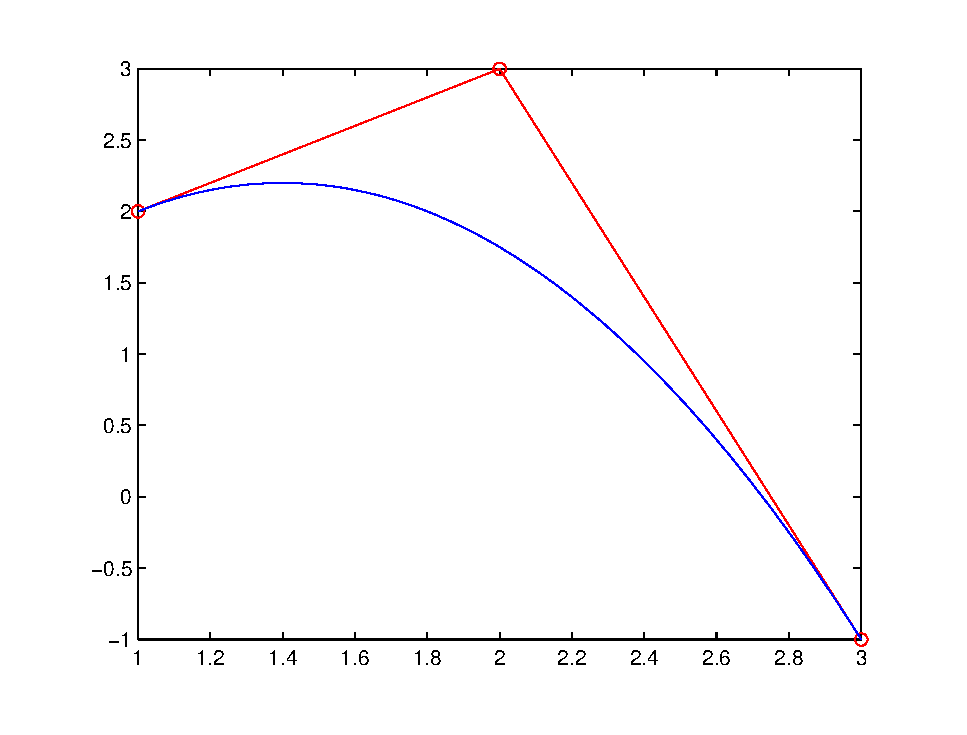
\includegraphics[width=6.8cm]{bezier3p.eps}} \qquad 
\subfigure[Curvas equivalentes de 4 a 6 puntos / 4 to 6 points equivalent curves  \label{fig:bz2}]{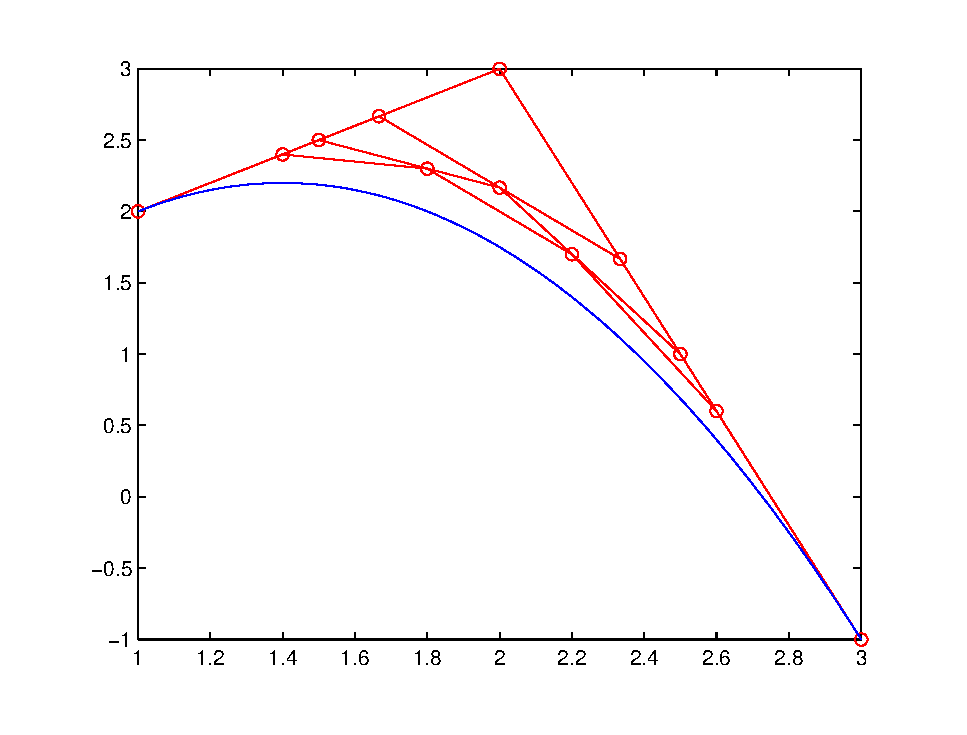
\includegraphics[width=6.8cm]{bezier6p.eps}}\\
\subfigure[Curvas equivalentes de 4 a 12 puntos / 4 to 12 points Equivalent curves   \label{fig:bz3}]{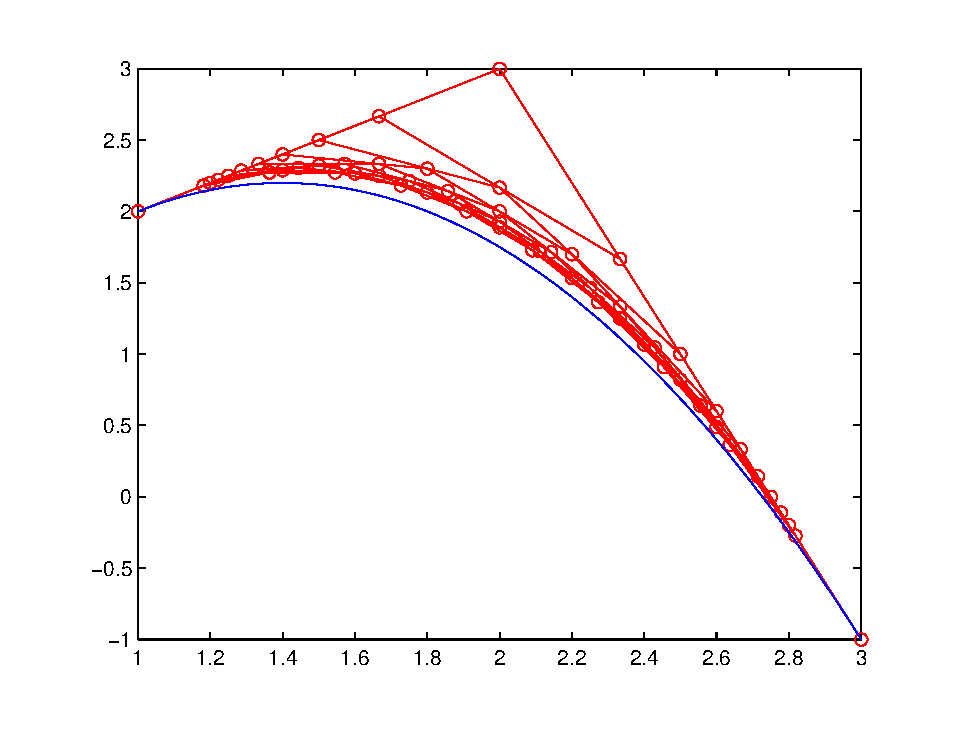
\includegraphics[width=6.8cm]{bezier12p.eps}} \qquad 
\subfigure[Curvas equivalentes de de 4 a 30 puntos / 4 to 30 points equivalent curve \label{fig:bz4}]{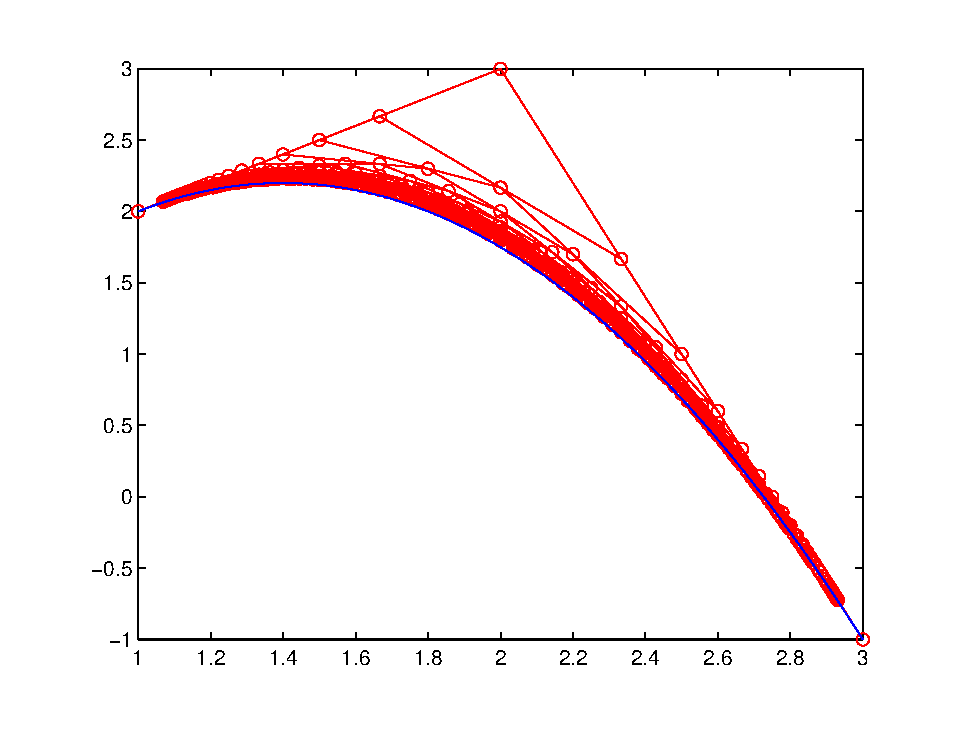
\includegraphics[width=6.8cm]{bezier30p.eps}}
\bicaption{Curvas de Bézier equivalentes, construidas a partir de una curva con tres puntos de control.}{Equivalent curves, built from a three control point Bézier's curve.} 
\label{fig:bzgrad}
\end{figure}
\begin{paracol}{2}
La función \mintinline{python}{bzeq} del módulo \mintinline{python}{bezier.py}, incluido más arriba  permite calcular la curva equivalente de Bézier a una dada, para cualquier número de puntos de control que se desee. \index{Curvas de Bézier equivalentes}
\paragraph{Derivadas.} Las derivadas de una curva de Bézier con respecto al parámetro $t$ son particularmente fáciles de obtener a partir de los puntos de control. Si tenemos una curva de Bézier de grado $n$, definida mediante puntos de control $\vec{p}_i$. Su derivada primera con respecto a $t$ será una curva de Bézier de grado $n-1$, cuyos puntos de control $\vec{d}_i$  puede obtenerse como:

\switchcolumn
Function \mintinline{python}{bzeq} in \mintinline{python}{bezier.py} module above include, allows us to calculate the Bezier's curve equivalent to any other given, using any number of control points. \index[eng]{Equivalent Bezier's curves}



\paragraph{Derivatives.} To compute the derivatives of a Bezier's curve  with respect to parameter $t$ is particularly easy, using the control points. Suppose we have a degree $n$ Bezier's curve, defined from control points $\vec{p}_i$. It first derivative with respect to $t$ will be a Bezier's curve of degree $n-1$, whose control point we can compute as: 
\end{paracol}

\begin{equation*}
\vec{d_i} = n\left(\vec{p_{i+1}} -\vec{p_i}\right)
\end{equation*}
\begin{paracol}{2}
La nueva curva de Bézier obtenida de este modo, es una hodógrafa; representa el extremo de un vector tangente en cada punto a la curva de Bézier original  y guarda una relación directa con la velocidad a la que se recorrería dicha curva. \index{hodógrafa}

La figura \ref{fig:bzc}, muestra una curva de Bézier sobre la que se ha trazado el vector derivada para algunos puntos. La figura \ref{fig:bzd} muestra la hodógrafa correspondiente y de nuevo los mismos vectores derivada de la figura \ref{fig:bzc}

La función \mintinline{python}{dbez}, incluida en el módulo \mintinline{python}{bezier.py} permite calcular los puntos de control de la derivada de una curva de Bézier.

\switchcolumn
The new Bézier curve we obtain is a hodograph. It represents the position of the tips of vectors tangent in each point to the original Bézier curve and has a direct relationship with the speed at which you can travel across the curve at any point.

Figure \ref{fig:bzc} shows a Bezier's curve an the derivative vector at some points of the curve. Figure \ref{fig:bzd} show the hodograph corresponding to and the same derivative vectors of de curve presented in figure \ref{fig:bzc}  

Function \mintinline{python}{dbez}, belonging to the module \mintinline{python}{bezier.py} included above, allows us to compute  the derivative of any Bezier's curve.
\end{paracol}

\begin{figure}[h]
\centering
\subfigure[Curva de Bézier (4 puntos) / Bézier's curve (4 points) \label{fig:bzc}]{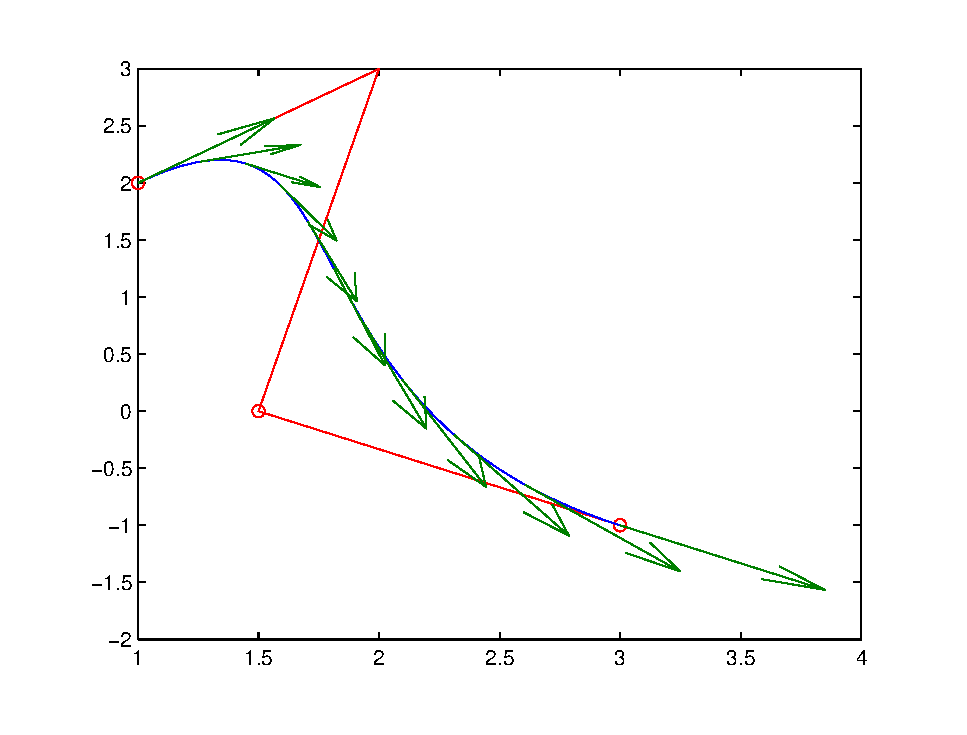
\includegraphics[width=7cm]{bezierder.eps}} \qquad 
\subfigure[Derivada (hodógrafa) / Derivative (hodograph) \label{fig:bzd}]{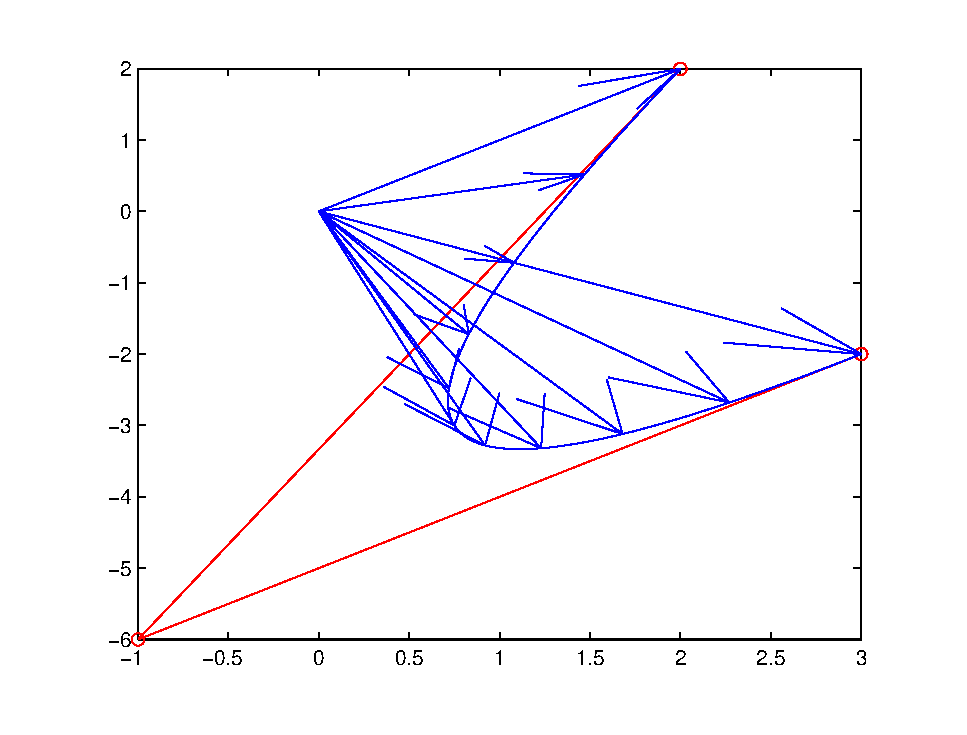
\includegraphics[width=7cm]{bezierhodg.eps}}
\bicaption{Curva de Bézier y su derivada con respecto al parámetro del polinomio de Bernstein que la define: $t \in [0,1]$}{Bézier's curve and its derivative with respect to the Berstein's polynomial parameter which defines the curve $ t \in [0,1]$} 
\label{fig:bzder}
\end{figure} 

\begin{paracol}{2}
\paragraph{Interpolación con curvas de Bézier} Podemos emplear curvas de Bézier para interpolar un conjunto de puntos $\lbrace \vec{p}_0, \cdots  \vec{p}_m\rbrace$. Si empleamos un curva para interpolar cada par de puntos, $\vec{p}_i, \vec{p}_{i+1}, \; i =1, \cdots m-1$ tenemos asegurada la continuidad en los puntos interpolados puesto que las curvas tienen que pasar por ellos. Como en el caso de la interpolación mediante splines, podemos imponer continuidad en las derivadas para conseguir una curva de interpolación suave. En el caso de las curvas de Bézier esto es particularmente simple. Si llamamos $B$ a la curva de Bézier de grado $n$ construida entre los puntos $\vec{p}_{i-1}, \vec{p}_{i}$  con puntos de control, $\vec{p}_{i-1}, b_1, \vec{b}_2,\cdots, \vec{b}_{n-1},\vec{p}_{i}$, y  $C$ a la curva de Bézier de grado $s$ construida entre los puntos $\vec{p}_{i}, \vec{p}_{i+1}$  con puntos de control, $\vec{p}_{i}, \vec{c}_1, \vec{c}_2,\cdots, \vec{c}_{s-1},\vec{p}_{i+1}$. Para asegurar la continuidad en la primera derivada en el punto $\vec{p_i}$ basta imponer,

\switchcolumn
\paragraph{Interpolation using Bézier's curves} We can use Bézier's curve for interpolating a set of points, $\lbrace \vec{p}_0, \cdots  \vec{p}_m\rbrace$. If we use a curve to interpolate every pair of consecutive points, $\vec{p}_i, \vec{p}_{i+1}, \; i =1, \cdots m-1$ we assure the continuity in the interpolated points because the curves have necessarily to pass through them. As in the case of spline interpolation, we can also impose continuity to the derivatives to get a smooth interpolating curve. In the case of Bèzier's curves, this is especially simple. If we call $B$ to the $n$-degree Bezier's curve built between the points $\vec{p}_{i-1}, \vec{p}_{i}$  with control points, $\vec{p}_{i-1}, b_1, \vec{b}_2,\cdots, \vec{b}_{n-1},\vec{p}_{i}$, and $C$ to the $s$-degree Bezier's curve built between the points $\vec{p}_{i}, \vec{p}_{i+1}$  with control points, $\vec{p}_{i}, \vec{c}_1, \vec{c}_2,\cdots, \vec{c}_{s-1},\vec{p}_{i+1}$; we can assure the continuity of the first derivative in the point $\vec{p_i}$ just imposing that,   
\end{paracol}
\begin{equation*}
n\cdot\left(\vec{p}_i-\vec{b}_{n-1}\right) = s\cdot\left(\vec{c}_1-\vec{p}_i\right)
\end{equation*}
\begin{paracol}{2} 
Esta condición impone una relación entre el penúltimo punto de control de la curva $B$ y el segundo punto de control de la curva $C$. Pero deja completa libertad sobre el resto de los puntos de control elegidos para construir las curvas.

Podemos, por ejemplo, elegir libremente todos los puntos de control de la curva $B$ y obtener a partir de ella el punto $\vec{c}_1$,

\switchcolumn
This condition imposes a link between the second-last control point of the curve $B$ and the second control point of the curve $C$. However, it allows free election of the remaining control points to build the curves as desired.

For instance we can freely choose all control points of curve $B$ and use it to compute the point $\vec{c}_1$,
\end{paracol}
\begin{equation*}
\vec{c}_1 = \frac{n+s}{s}\vec{p}_i - \frac{n}{s}\vec{b}_{n-1}
\end{equation*}
\begin{paracol}{2}
	La figura \ref{fig:ibz3} muestra un ejemplo de interpolación en la que se ha aplicado la condición de continuidad en la derivada que acabamos de describir.
	
	\switchcolumn
	Figure \ref{fig:ibz3} shows an example of interpolation in which we have applied the derivative continuity condition we have described. 
\end{paracol}

\begin{figure}[h]
\centering
\subfigure[Interpolación mediante curvas de Bézier de 3 puntos / Interpolation using three control points Bezier's curves) \label{fig:ibz}]{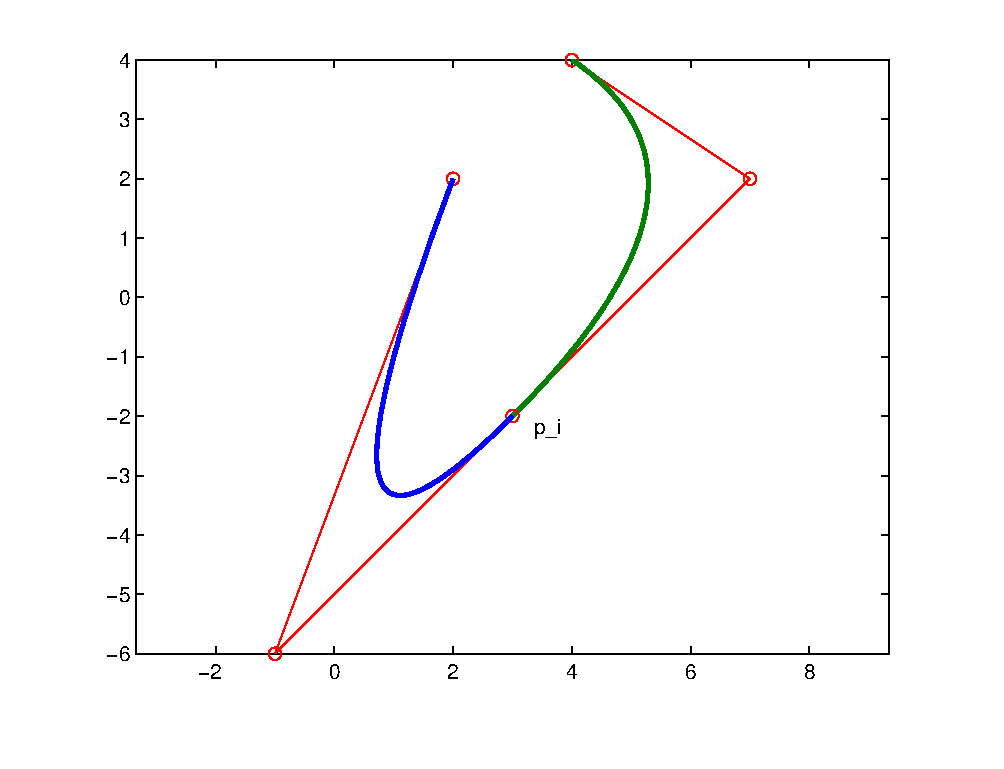
\includegraphics[width=7cm]{bezierint.eps}} \qquad 
\subfigure[Interpolación mediante curvas de Bézier de 3 y 4 puntos / iNterpolation using 3 and 4 control points Beziers's curves   \label{fig:ibz2}]{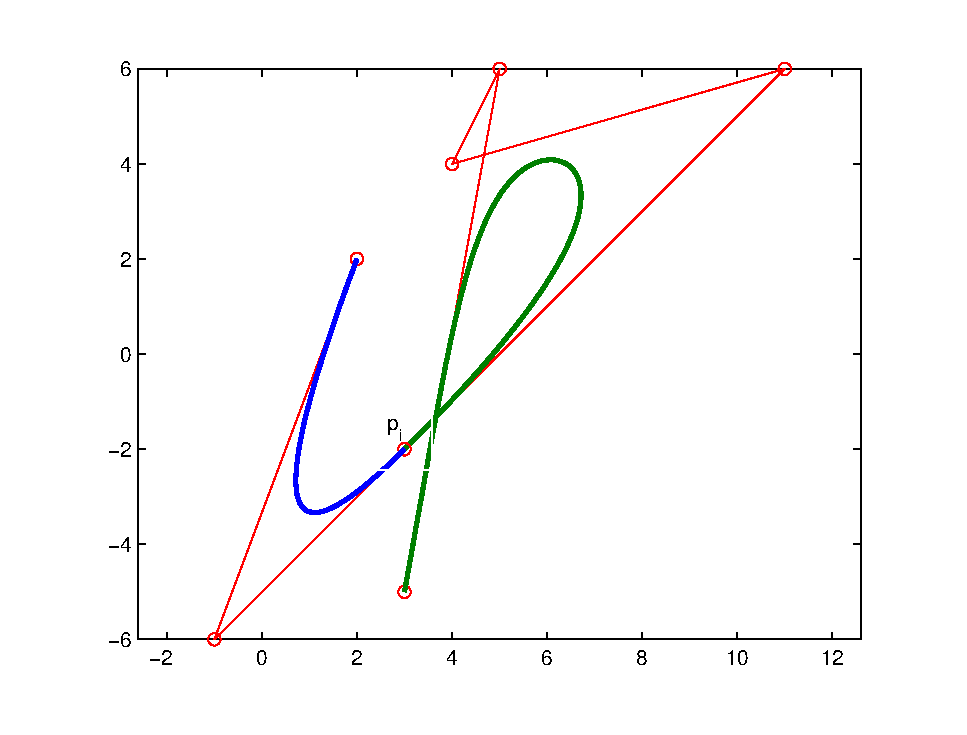
\includegraphics[width=7cm]{bezierint2.eps}}
\bicaption{Interpolación de tres puntos mediante dos curvas de Bézier}{interpolating three point using two Bezier's curves} 
\label{fig:ibz3}
\end{figure}
 \begin{flalign*}
 	&& \Biggr \}\reversemathwitch*    
 \end{flalign*}
\newpage
\begin{paracol}{2}
\section{ejercicios}
\begin{enumerate}
\item Carga en python los datos del fichero \texttt{datos.txt}\footnote{disponible en \url{https://github.com/UCM-237/LCC/tree/master/datos}} y realiza las siguientes tareas:
\begin{enumerate}
\item \label{ej1a} Crea una función que a partir de dos vectores de datos $x,y$ de igual longitud $n+1$, calcula la matriz de Vandermonde necesaria   para obtener el polinomio de interpolación asociado a los puntos. Empleando la primera columna de datos contenida en \texttt{datos.txt} como datos $x$ y la segunda como datos $y$, genera el polinomio de interpolación,
\begin{equation*}
p(x)=a_0+a_1x+a_2x^2+\cdots+a_nx^n
\end{equation*}

Calcula el valor que toma el polinomio de interpolación en 100 puntos equiespaciados entre los valores $x_0$ y $x_{n}$ de los datos del fichero. Dibuja en una misma gráfica los resultados obtenidos, empleando una línea continua, y los valores del fichero, mediante puntos separados empleando el símbolo que prefieras. Comprueba que el polinomio pasa por los puntos contenidos en el fichero.

\item Reproduce en python la función 'Lagrange' de la sección \ref{sec:lagranje} para calcular el polinomio interpolador de Lagrange. Emplea la función que acabas de crear para recalcular los valores del polinomio de interpolación realizado en el ejercicio anterior y comprueba que los resultados obtenidos son los mismos que empleando la matriz de Vandermonde.

\item A partir de los ejemplos de la sección  sección \ref{sec:difdiv}, crea un programa que calcule los coeficientes del polinomio interpolador de diferencias divididas a partir de dos vectores de datos  $x,y$ de igual longitud $n+1$ y un segundo programa que calcule el valor del polinomio en un punto cualquiera a partir de los coeficientes obtenidos con el primer programa. Vuelve a calcular, empelando ahora el polinomio de diferencias dividas, los valores del polinomio de interpolación sobre los mismos datos empleados en los ejercicios anteriores y comprueba que da los mismos resultados.

\item Por último, crea una función que calcule el polinomio de interpolación de Newton-Gregory (sección \ref{sec:newgre}). ¿Es posible usarlos para interpolar los datos del archivo\\ \texttt{datos.txt}? Si la respuesta el afirmativa, repite el cálculo del polinomio de interpolación, empleando Newton-Gregory y comprueba si coincide con lo obtenido en los ejercicios anteriores.

\item Usa la función de numpy \mintinline{python}{interp1d} y emplea de nuevo los datos del fichero \texttt{datos.txt}, para obtener el resultado de interpolar los valores en 100 puntos equiespaciados entre los valores $x_0$ y $x_{n}$ del fichero.  Emplea para ello los métodos \texttt{'nearest'} y \texttt{'linear'}. Repite el cálculo empleando ahora la función de numpy  \texttt{'CubicSpline'}. Dibuja los resultados en la misma gráfica empleada en el ejercicio  \ref{ej1a})
\end{enumerate}
\item Construye a partir del código de ejemplo de la sección \ref{sec:mc}, una función que calcule el polinomio de grado $n$ que ajusta por mínimos cuadrados un conjunto de pares de datos $(x, y)$. Pruébalo sobre los datos del fichero \texttt{datos.txt}, sin emplear pesos. Compara los coeficientes del polinomio obtenido con los que se obtienen empleando la función \texttt{Polynomial.fit} de Numpy. ¿Qué conclusión sacas?

\item Añade el código necesario al programa anterior para que, una vez obtenidos los coeficientes del polinomio de mínimos cuadrados, la función calcule y devuelva un vector $r$ con los valores de los residuos, $r = y -p(x)$, donde $x$ e $y$ son los vectores del conjunto de datos para los que se ha obtenido el polinomio de mínimos cuadrados y $p$ los valores obtenidos aplicando el polinomio a los valores $x$ de la colección de datos.
\end{enumerate}
\switchcolumn
\section{exercises}
\begin{enumerate}
	\item Load in Python the date held in file\\ \mintinline{python}{datos.txt}\footnote{available in \url{https://github.com/UCM-237/LCC/tree/master/datos}} an carry out the following tasks:
\begin{enumerate}
	\item Build a function that taking two data vector, $x$, $y$ of the same length, $n+1$, computes the Vandermonde's matrix needed for obtaining the interpolating polynomial associated to the points. Using the first data column in \mintinline{python}{data.txt} as $x$ and the second column as $y$ compute the the interpolating polynomial,
	\begin{equation*}
		p(x)=a_0+a_1x+a_2x^2+\cdots+a_nx^n
	\end{equation*}
	
	Compute the values of the interpolating polynomial in 100 equispaced points between values $x_0$ and $x_{n}$ of the data file. In the same gra\-phic, draw the results obtained using a continuous line and the file data as single points, using the symbol you prefer. Check that the polynomial passes through the data point included in the file.
	
	\item Write the 'Lagrange' function for computing the Interpolating Lagrange polynomial in Python, included in section \ref{sec:lagranje}. Use the function you just created to recompute the values of the interpolating polynomial obtained in the previous exercise and check that you get the same results as using Vandermonde's matrix.
	
	\item Departing from the examples in section \ref{sec:difdiv}, build a program for computing the divided differences polynomial coefficients, usin two data arrays $x$ and $y$ with the same length, $n+1$. Buid also a second program for computing the value of the polynomial in any point, using the coefficients computed with the previous program. Recompute one more time, now using the divided differences polynomial the values of the interpolation polynomial, of the same data use in previous exercises. Check that you get the same results.
	
	\item Lastly, build a function that compute the Newton-Gregory's interpolating polynomials (section \ref{sec:newgre}). It is possible to interpolate the data held in the file \mintinline{python}{datos.txt} using the Newton-Gregory's polynomial? If the answer is 'yes', use your function just writen to repeat the computing of the intepolation polynomial carried out in previous section and check that the results meet those obtained in previous sections.
	
	\item Using the Numpy's function\\ \mintinline{python}{interp1d} and the data contained in file \mintinline{python}{datos.txt}, compute the result of interpolating in 100 equispaced points between values $x_0$ and $x_n$ of the file dataset. Do it using the method \texttt{'nearest'} and \texttt{'linear'}. Repeat the computing but now using the  Numpy function   \texttt{'CubicSpline'}. Draw the results in the same graphic where you drew exercise \ref{ej1a}) results.  
\end{enumerate}
\item create a function that calculates the $n$-degree polynomial using the least squared method to fit a set of data pairs $(x,y)$, using the code in section \ref{sec:mc} as a reference. Test your function with the data in the file \mintinline{python}{datos.txt} without employing weights. Afterward, compare the coefficients produced by your program with those obtained using the Numpy function \mintinline{python}{Polynomial.fit}. What conclusion can you draw from the comparison?

\item Add the necessary code to the previous program so that, once the coefficients of the least square polynomials has been obtained, the function calculates and return a vector $r$ with the values of the residuals, $r = y -p(x)$, where $x$ and $y$ are the data set for which the function has computed the least square polynomial and $p$ the values obtained applying the polynomial to the $x$ values of the data set.
\end{enumerate}
\end{paracol}
\begin{paracol}{2}
\section{Test del curso 2020/21}

\noindent \textbf{Problema 1}. Una cuerda de escalada aumenta su longitud cuando está sometida a una tensión estacionaria. En particular, el aumento de longitud sigue la siguiente ley
\begin{equation}\label{eq:0}
T = b\tanh(ax),
\end{equation}
donde $T \in \mathbb{R}^+$ es la tensión aplicada en Newtons, $x \in \mathbb{R}^+$ es la elongación de la cuerda en metros y $a, b \ \in \mathbb{R}^+$ son parámetros constantes que dependen de las características de la cuerda.

En función del comportamiento físico de la cuerda, podemos distinguir tres regímenes:

\begin{itemize}
	\item \emph{Comportamiento elástico}: Se dice que el comportamiento de la cuerda es elástico si al desaparecer la tensión la cuerda recupera su longitud original. Esto se cumple para tensiones estacionarias pequeñas, y las elongaciones están acotadas por un valor positivo $x_{le}$, esto es, $0 \le x \le x_{le}$. En régimen elástico, la ecuación (\ref{eq:0}) puede aproximarse por la siguiente expresión
\begin{equation}\label{eq:1}
T = \kappa x - \gamma x^3,
\end{equation}
donde $\kappa,\gamma \in \mathbb{R}^+$ son también constantes.

\item \emph{Comportamiento plástico}: Se dice que el comportamiento de la cuerda es plástico si al desaparecer la tensión la cuerda se deforma y no recupera su longitud original. Esto ocurre para tensiones medias, y la elongación alcanzada en este régimen está también acotada por $x_{le} < x \le x_{max}$.

\item \emph{Rotura}: Para tensiones grandes la cuerda no admite elongaciones mayores que $x_{max}$ y se rompe.

\end{itemize}

La fábrica de cuerdas de escalada \textit{Pa'bennos Matao S.L.} ha realizado un estudio sobre un nuevo modelo de cuerda. En dicho estudio se fijó un extremo de la cuerda a una mesa abatible suficientemente grande (que hará la función de un plano inclinado), y se ató el otro extremo de la cuerda a una pesa. De manera secuencial se fue incrementando el ángulo formado por la mesa con la horizontal. En particular, se empezó con cero grados y aumentando el ángulo hasta que finalmente la cuerda alcanzó $x_{max}$ y se rompió. 

Del estudio se pudo registrar la elongación sufrida por la cuerda por los distintos $i\in\{1,\dots,52\}$ ángulos de inclinación. Estos datos están en el archivo:  \texttt{cuerda.txt}\footnote{disponible en \url{https://github.com/UCM-237/LCC/tree/master/datos}}, en donde:
\begin{itemize}
	\item La primera columna corresponde a los ángulos $\theta_i$ medidos en radianes.
	\item La segunda columna corresponde a las elongaciones $x_i$ medidas en metros.
\end{itemize}

\begin{enumerate}
\item (\textbf{1 punto}) Estima el valor de la elongación $x_{max}$ para el cual se produce la rotura de la cuerda.

\item (\textbf{1 punto}) Obtén la tensión ejercida por la pesa sobre la cuerda para cada ángulo de inclinación $\theta_i$ de la mesa, esto es
\begin{equation} \label{eq:2}
T_i = mg\sin(\theta_i),
\end{equation}
donde $m =1000$ Kg y $g = 9.8$ m/s$^2$. Representa gráficamente los datos: $T_i$ frente a $x_i$.

\item A partir de los pares de datos $T_i$ y $x_i$ podemos estimar la ecuación (\ref{eq:1}).
\begin{enumerate}
\item (\textbf{2 puntos}) Ajusta los datos por mínimos cuadrados a un polinomio de grado tres. Dado que dicha aproximación solo es válida para el régimen de comportamiento elástico, es imprescindible realizar el ajuste del polinomio asignando pesos a cada par de datos. Para dar más valor a las elongaciones pequeñas y menos a las grandes, utiliza la siguiente expresión para definir los pesos
\begin{equation}
\omega_i = e^{-10x_i^2}.
\end{equation}
\item (\textbf{1 punto})  Representa, sobre la gráfica dibujada en el apartado 2a, el polinomio obtenido en el apartado 3a. Según tu criterio, ¿es razonable el ajuste realizado?
\end{enumerate}

\item (\textbf{1 punto})  Los coeficientes de las ecuaciones (\ref{eq:0}) y (\ref{eq:1}) están relacionados por las siguientes expresiones
\begin{equation}
\kappa = b\cdot a, \quad \gamma = \frac{b\cdot a^3}{3}. \nonumber
\end{equation}
		Calcula los valores de $a$ y $b$ a partir de los coeficientes del polinomio obtenido en el apartado 3a. Representa, en la misma gráfica de los apartados anteriores, la función $T(x) = b\tanh(ax)$. Explica, a la vista del gráfico, si los resultados obtenidos son razonables o no. 

\item (\textbf{1 punto}) Calcula el valor de los residuos $r_i = T_i - P_3(x_i)$, donde $P_3(x)$ es el polinomio de grado tres obtenido en el apartado 3a. Si la cota $x_{le}$ para el comportamiento elástico de la cuerda viene definida cuando $r_i \approx 500 N$. Encuentra un valor aproximado para $x_{le}$. \\
\textbf{Nota:} Hay que buscar $x_{le}$ empleando código. No vale dibujar los residuos y estimarlo a vista.
\end{enumerate}

\switchcolumn
\section{Course 2020/21 test}
\noindent \textbf{Question 1.} A Climbing rope stretches when it suffers a stationary strain. Specifically, the increase in length follows the following law,

\begin{equation}\label{eq:0}
	T = b\tanh(ax),
\end{equation}
Where $T \in \mathbb{R}^+$ is the applied strain in Newtons, $x \in \mathbb{R}^+$ is the rope stretching in meters and  $a, b \ \in \mathbb{R}^+$ are constant parameter which depend on the rope characteristics.

According to the rope physical behaviour, we can observe three regimes.

\begin{itemize}
	 \item \emph{elastic behaviour}: The rope follows an elastic behaviour if it recovers its original length once we withdraw the strain. This is the normal behaviour under small stationary strains. In this case, the stretching is upper bounded by a positive value $x_{le}$, that is, $0 \le x \le x_{le}$. In the elastic regime equation \label{eq:0} can be approximated by the following expression,
	
	\begin{equation}\label{eq:1}
		T = \kappa x - \gamma x^3,
	\end{equation}
	where $\kappa, \gamma \in \mathbb{R}^+$ are also constant.
	
	\item \emph{Plastic behaviour:} The rope behaviour is considered plastic if the rope deforms after removing the strain and does not recover its original length. This behaviour takes place for intermediate strains and, in this plastic regime, the rope stretching is also bounded between two limits $x_{le} < x \le x_{max}$ .
	
	\item \emph{Breaking off:} The rope does not admit a bigger stretching and breaks off for larger strains.
\end{itemize}

 The climbing ropes company \emph{Slink Yer Hook, ltd.} conducted a study on a new brand of rope. They attached one end of the rope to a tilting table, which was used as an inclined plane, and the other to a weight for the study. The angle between the table and the horizontal was gradually increased. The test started with a zero-degree angle, and the angle was increased until the rope reached the length $x_{max}$ and broke.
 
During the study, the stretching suffered by the rope for different tilting angles $i \in \{1,\cdots,52\}$ was registered. These data are available in the file \texttt{cuerda.txt}\footnote{Available in \url{https://github.com/UCM-237/LCC/tree/master/datos}}, where:

\begin{itemize}
	\item The first column holds the angles $\theta_i$ measured in radians.
	\item The second column holds the elongations $x_i$ measured in meters.
\end{itemize}

\begin{enumerate}
	\item (\textbf{1 point}) Estimate the stretching limit value $x_{max}$ beyond which the rope breaks.
	
	\item (\textbf{1 point}) compute the strain exerted to the rope for the weight at any table tilting angle $\theta_i$, that is,
	 \begin{equation} \label{eq:2}
	 	T_i = mg\sin(\theta_i),
	 \end{equation}
	 where  $m =1000$ Kg and $g = 9.8$ m/s$^2$. Draw a  $T_i$ vs $x_i$ graph.
	 \item From data pairs $T_i$ and $x_i$ we can estimate equation  (\ref{eq:1}).
	 \begin{enumerate}
	 	\item (\textbf{2 points})To fit the data, utilize a three-degree least squares polynomial. Because this method is only suitable for elastic behavior, it's important to assign weights to the data when calculating the polynomial. Use the following expression to define the weights, which will enhance the influence of small elongations and reduce the impact of larger ones.
	 	\begin{equation}
	 		\omega_i = e^{-10x_i^2}.
	 	\end{equation}
	 	\item (\textbf{1 point}) Plot on top the graph drew in question 2a, the polynomial you have computed in question 3b. Is it reasonable the fitting carried out? explain why.
	 \end{enumerate}
	 \item (\textbf{1 point}) Coefficient in equations  (\ref{eq:0}) y (\ref{eq:1}) are related by the following expressions,
	 \begin{equation}
	 	\kappa = b\cdot a, \quad \gamma = \frac{b\cdot a^3}{3}. \nonumber
	 \end{equation}
	 Compute the values of parameters $a$ and $b$ departing from the coefficients of the polynomial obtained in question 3a. Plot the function $T(x) = b\tanh(ax)$ in the same graphic used in the previous questions. Explain, according to the graphic, is the results achieved are reasonable or not.
	 \item (\textbf{1 point}) Compute the value of residuals $r_i=T_i-P_3(x_i)$ where $P_3(x)$ is the polynomial obtained in question 3a. Suppose that the limit $x_{le}$ for the rope elastic behaviour is reached when $r_i \approx 500 N$, Find an approximated value for $x_{le}$.\\
	 \textbf{Note:} It is not enough to draw the residuals and estimate $x_{le}$ by simple inspection. You must use code to do it.	     
\end{enumerate}
\end{paracol}
\begin{paracol}{2}
\noindent \textbf{Problema 2.} Dados los siguiente valores de la función $f(x)$:
\switchcolumn
\noindent \textbf{Problem 2.} Given the following values belonging to function $f(x)$:
\end{paracol}

\begin{equation}
	f(0) = 1, \quad f \left(\frac{\pi}{4}\right)= \frac{\sqrt{2}}{2}, \quad f \left(\frac{\pi}{2}\right) = 0, \quad f \left(\frac{3\pi}{4}\right) = -\frac{\sqrt{2}}{2}, \quad f(\pi) = -1 \nonumber
\end{equation}

\begin{paracol}{2}
\begin{enumerate}
	\item (\textbf{1.5 puntos}) Utilizando el comando de Numpy correspondiente, obtener mediante interpolación con splines cúbicos los valores de la función $f(x)$ sobre cien puntos equiespaciados en el intervalo $[0,\pi]$.
	
	\item (\textbf{1.5 puntos}) Dibuja mediante un diagrama de barras las differencias entre los $f(x)$ y la función $\cos(x)$ de Python en los mismos puntos del intervalo anterior. Considera que no necesitamos más de dos decimales para la precisión el cálculo de la función coseno; ¿podríamos utilizar la interpolación para $f(x)$?
\end{enumerate}
\switchcolumn
\begin{enumerate}
	\item (\textbf{1.5 points}) Using an appropriate Numpy function, compute using cubic splines interpolation the values of function $f(c)$ at 100  equispaced points into the interval $[0,\pi]$.
	
	\item (\textbf{1.5 points})  Use a bar plot to draw the differences between $f(x)$ and the function $\cos(x)$ in the same points interpolated in the previous question. Suppose we only need up to two decimal precisions to calculate the cosine function. Could we then use the interpolation calculated for $f(x)$?    
\end{enumerate}
\end{paracol}

